% -*- TeX -*- -*- UK -*-
% ----------------------------------------------------------------
% arXiv Paper ************************************************
%
% Subhaneil Lahiri's template
%
% Before submitting:
%    Comment out hyperref
%    Comment out showkeys
%    Replace \input{mydefs.tex} with its contents
%       or include mydefs.tex in zip/tar file
%    Replace \input{newsymb.tex} with its contents
%       or include newsymb.tex in zip/tar file
%    Put this file, the .bbl file, any picture or
%       other additional files and natbib.sty
%       file in a zip/tar file
%
% **** -----------------------------------------------------------
\documentclass[12pt]{article}
%Preamble:
\usepackage{a4wide}
\input{sl_preamble.tex}
\input{sl_graphics_preamble.tex}
\graphicspath{{"Figures/"}}
%
% >> Only for drafts! <<
\usepackage[notref,notcite]{showkeys}
% ----------------------------------------------------------------
%\numberwithin{equation}{section}
%\renewcommand{\baselinestretch}{1.5}
% ----------------------------------------------------------------
% New commands etc.
\input{sl_definitions.tex}
\input{sl_symbols.tex}
%matrices
\newcommand{\inv}{^{-1}}
\newcommand{\dg}{^\mathrm{dg}}
\newcommand{\trans}{^\mathrm{T}}
\newcommand{\I}{\mathbf{I}}
%vec of ones
\newcommand{\onev}{\mathbf{e}}
%mat of ones
\newcommand{\onem}{\mathbf{E}}
%Markov matrix
\newcommand{\MM}{\mathbf{Q}}
%equilibrium distribution
\newcommand{\pr}{\mathbf{p}}
\newcommand{\eq}{\pr^\infty}
%first passage times
\newcommand{\fpt}{\mathbf{T}}
%off-diag first passage times
\newcommand{\fptb}{\overline{\fpt}}
%fundamental matrix
\newcommand{\fund}{\mathbf{Z}}
%other symbols
\newcommand{\Pb}{\mathbf{P}}
\newcommand{\D}{\mathbf{D}}
\newcommand{\pib}{\boldsymbol{\pi}}
\newcommand{\Lb}{\boldsymbol{\Lambda}}
\newcommand{\w}{\mathbf{w}}
\newcommand{\W}{\mathbf{W}}
\newcommand{\frg}{\W^\mathrm{F}}
\newcommand{\M}{\mathbf{M}}
\newcommand{\F}{\boldsymbol{\Phi}}
\DeclareMathOperator{\SNR}{SNR}
\newcommand{\CS}{\mathcal{S}}
\newcommand{\CA}{\mathcal{A}}
\newcommand{\CB}{\mathcal{B}}
\newcommand{\comp}{^\mathrm{c}}
\newcommand{\pot}{^{\text{pot}}}
\newcommand{\dep}{^{\text{dep}}}
\newcommand{\potdep}{^{\text{pot/dep}}}
\newcommand{\norm}{_0}
\newcommand{\inc}{_{\text{inc}}}
\newcommand{\dec}{_{\text{dec}}}
\newcommand{\incdec}{_{\text{inc/dec}}}
\newcommand{\wt}{_{\text{WT}}}
\newcommand{\ko}{_{\text{D$^\mathrm{b}$K$^\mathrm{b}$-/-}}}
\newcommand{\KO}{D$^\mathrm{b}$K$^\mathrm{b}$-/-}
\newcommand{\tpre}{t_{\text{pre}}}
\newcommand{\ttrain}{t_{\text{train}}}
\newcommand{\lmax}{_{\text{max}}}
\newcommand{\lmin}{_{\text{min}}}
% ----------------------------------------------------------------
%
%%%%%%%%%%%%%%%%%%%%%%%%%%%%%%%%%%%%%%%%%%%%%%%%%%%%%%%%%%%%%%%%%%%%%%%%%%
% Title info:
\title{Models of VOR learning in MHC knockout mice}
%
% Author List:
%
\author{Subhaneil Lahiri
%
}

\begin{document}

\maketitle


%%%%%%%%%%%%%%%%%%%%%%%%%%%%%%%%%%%%%%%%%%%%%%%%%%%%%%%%%%%%%%%%%%%%%%%%%%


\begin{abstract}
  We see if we can model VOR gain increase and decrease learning in mice with a knockout in MHC as well as wild-type.
\end{abstract}

\tableofcontents

%%%%%%%%%%%%%%%%%%%%%%%%%%%%%%%%%%%%%%%%%%%%%%%%%%%%%%%%%%%%%%%%%%%%%%%%%%
% Beginning of Article:
%%%%%%%%%%%%%%%%%%%%%%%%%%%%%%%%%%%%%%%%%%%%%%%%%%%%%%%%%%%%%%%%%%%%%%%%%%

\section{Introduction and summary}\label{sec:intro}




\section{The setup}\label{sec:setup}


\subsection{Models of synapses}\label{sec:synapse}

We make the following assumptions:
\begin{itemize}
  \item There are $N$ identical synapses with $M$ internal functional states.
  \item The states of different synapses are independent of each other.
  \item The synapses that are eligible for plasticity are chosen randomly.
  \item The potentiating/depressing plasticity event timings are distributed as Poisson processes with rates $rf\potdep$, where $f\pot+f\dep=1$.
  \item Potentiation and depression are described by Markov processes with transition probabilities $\M\potdep$.
  \item The synaptic weights of the internal states are given by the column vector $\w$. This can only take two values that we can call $\pm1$, except for the pooled resource model that we will discuss in \sref{sec:pooledmodel} and \sref{sec:pooled}.
\end{itemize}

The independence and identicalness of synapses means that the state of the system can be completely described by the probability distribution of the internal states, the row vector $\pr(t)$.

The evolution of this probability is described by a forgetting matrix, $\frg$:
%
\begin{equation}\label{eq:evolve}
  \diff{\pr(t)}{t} = r\pr(t)\frg,
  \qquad
  \frg = f\pot\M\pot+f\dep\M\dep-\I.
\end{equation}
%
Eventually, this will settle into the equilibrium distribution:
%
\begin{equation}\label{eq:eqprob}
  \eq\frg=0.
\end{equation}
%



With only two possible synaptic weights, the distribution of synaptic weights is completely described by the mean, $\pr(t)\w$.


\subsection{Model of VOR learning experiment}\label{sec:learning}

Training the animal will not change the internal dynamics of a synapse under potentiation or depression.
It will change the environment, will lead to a change in how often potentiation and depression occur.
It could be manifested in a change in which synapses are potentiated/depressed, but this could not be captured in this type of model.
We will model this by changing $f\potdep$, leaving $r$ and $\M\potdep$ unchanged.

The untrained case will be described by $f\pot=f\pot\norm$.
Gain-increase training  will be described by $f\pot=f\pot\inc<f\pot\norm$, and
gain-decrease training  will be described by $f\pot=f\pot\dec<f\pot\norm$. Note that the forgetting matrix \eqref{eq:evolve} and the equilibrium distribution \eqref{eq:eqprob} depends on $f\pot$, which we will indicate with subscripts.

Before training, the synaptic distribution will in equilibrium with $f\pot\norm$.
During gain-increase training, it will evolve according to \eqref{eq:evolve} with $f\pot\inc$:
%
\begin{equation}\label{eq:nopre}
  \pr(t) = \eq\norm \exp\prn{rt\frg\inc}.
\end{equation}
%
On the other hand, if the gain-increase training follows gain-decrease pre-training for some time period, $\tpre$:
%
\begin{equation}\label{eq:withpre}
  \pr(t) = \eq\norm \exp\prn{r\tpre\frg\dec} \exp\prn{r(t-\tpre)\frg\inc}.
\end{equation}
%

We will describe the effect of training by the decrease in mean synaptic weight:
%
\begin{equation}\label{eq:learning}
  L(t) = \prn{\pr(0)-\pr(t)}\w.
\end{equation}
%
The behavioural output (VOR gain) will be some non-linear function of the synaptic weights, so the best we can hope for is to reproduce qualitative features of the experiment.

The MHC mutant has a lower threshold for depression.
We can model this by changing $\W\dep\wt$ to $\W\dep\ko$, which should have larger matrix elements.

QUESTION: Should $f\pot\wt=f\pot\ko$?

If they are equal, this would change the mean synaptic weight in equilibrium.
This seems like it would affect the ability of the network to perform its function, and one might expect adaptation to the environment to produce an equilibrium state that has the same performance.
In any case, if the synaptic weights are different, the electrical activity will be different, and there will be no reason to expect the same statistics for potentiation or depression.

On the other hand, one could imagine adjusting $f\pot\wt$ and $f\pot\ko$ so that $\eq\wt\w = \eq\ko\w$.
But, now that the synaptic weights are the same, the electrical activity will be the same, and there will be no reason to expect different statistics for potentiation or depression.
If we did this for the multistate or two-state models, we'd remove all differences between the wild-type and \KO\ mutant.


\section{Simulations}\label{sec:sims}

\subsection{Models and parameters}

We will look at three different models, the cascade model (see \cite{Fusi2005cascade} and \autoref{fig:models}\ref{fig:cascade}), the multistate model (see \cite{amit1994learning,Fusi2007multistate} and \autoref{fig:models}\ref{fig:multistate}) and the two-state model (which can be thought of as a special case of the previous two, see \autoref{fig:models}\ref{fig:binary}).

For the cascade model, we will use the same value for the parameter $x$ (which controls the decay of transition rates, see \cite{Fusi2005cascade}) for potentiation and depression in the wild-type as well as potentiation in the \KO\ mutant.
We will use a larger value for $x$ for depression in the \KO\ mutant.

For the multistate and two state models, we will use the same value for the transition probabilities, $q$ for potentiation and depression in the wild-type as well as potentiation in the \KO\ mutant.
We will use a larger value for $q$ for depression in the \KO\ mutant.

In each case, we set $f\pot\norm=\half$, $f\pot\inc=f\pot\norm+\Delta f$ and $f\pot\dec=f\pot\norm-\Delta f$. The values of all these parameters are listed in \autoref{tab:params}.

\begin{figure}
 \begin{center}
 \begin{myenuma}
  \item\aligntop{\includegraphics[height=2cm]{cascade.svg}}\label{fig:cascade}\hspace{0.5cm}
  \item\aligntop{\includegraphics[height=1.7cm]{multistate.svg}}\label{fig:multistate}\hspace{0.5cm}
  \item\aligntop{\includegraphics[height=1.7cm]{binary.svg}}\label{fig:binary}
 \end{myenuma}
 \end{center}
  \caption{Transition probabilities for different models.
  (\ref{fig:cascade}) In the cascade model, the transition probabilities decay geometrically with a parameter $x$ (see \cite{Fusi2005cascade}).
  (\ref{fig:multistate}) In the multistate model the transition probabilities for potentiation/depression are all equal and it is parameterised by these two values.
  (\ref{fig:binary}) The two-state model is parameterised by the two transition probailities.} \label{fig:models}
\end{figure}

\begin{table}
 \begin{center}
  \begin{tabular}{|l|c|c|c|c|c|c|}
    \hline
    % after \\: \hline or \cline{col1-col2} \cline{col3-col4} ...
    Model & \# states & pot,WT dep & \KO\ dep & $\Delta f$ & $r\ttrain$ & $r\tpre$ \\
    \hline
    Cascade    & 10 & $x=0.25$ & $x=0.33$ & -0.3 & 50 & 50 \\
    Cascade    & 10 & $x=0.25$ & $x=0.33$ & -0.3 & 50 & 150 \\
    Multistate & 10 & $q=0.6$  & $q=0.8$  & -0.1 & 50 & 50 \\
    Multistate & 10 & $q=0.6$  & $q=0.8$  & -0.4 & 20 & 20 \\
    Two-state  & 2  & $q=0.4$  & $q=0.8$  & -0.1 & 5 & 5 \\
    \hline
  \end{tabular}
 \end{center}
  \caption{Parameters used in simulations.} \label{tab:params}
\end{table}

\subsubsection{Pooled resource model}\label{sec:pooledmodel}

Suppose that there is some resource required for potentiation/depression that is shared between $P$ synapses and is depleted as more synapses are potentiated/depressed.
We can avoid going beyond the independent synapse model by modelling this pool of synapse as a single pseudo-synapse.

We will model the individual synapses with the two-state model. 
Let $i$ be the number of them that are potentiated.
We will model the effect of resource depletion linearly with the potentiation/depression probabilities for the individual synapses:
%
\begin{equation}\label{eq:depletion}
  \begin{aligned}
    q\pot &= \frac{(P-i-1)q\lmax + i\,q\lmin}{P-1}, \qquad
    q\dep &= \frac{(i-1)q\lmax + (P-i)q\lmin}{P-1}.
  \end{aligned}
\end{equation}
%
At each plasticity event for the pseudo-synapse, one of the individual synapses will be chosen randomly for update.
This effectively reduces the transition probabilities by $1/P$.

This pseudo-synapse would seem to have $2^P$ internal states.
However, we need only keep track of the number of potentiated synapses, not their identity, leaving $M=P+1$ states.
The transition network topology will then have a multistate toplogy (see \autoref{fig:models}\ref{fig:multistate}) but the transition probabilities will no longer be uniform and the weight of the pseudo-synapse is the mean of its constituent synapses:
%
\begin{equation}\label{eq:pooledweight}
  \w_i = \frac{2i}{P}-1.
\end{equation}
%


The Markov process is lumpable \wrt this partition of states (see \cite[\S6.3]{kemeny1960finite} for the discrete time version and \cite{burke1958markovian,Ball1993Lumpability} for continuous time).
The transition probabilities between lumps $i$ and $j$ is computed by choosing one state from lump $i$ and summing the transition probabilities to all states in lump $j$.
The result must be the same for all states in lump $i$.

For any state in lump $i$, there are $P-i$ synapses that can be potentiated to go to lump $i+1$.
Each of these transition probabilities is $q\pot/P$.
Similarly, there are $i$ synapses that can be depressed to go to lump $i-1$.
Each of these transition probabilities is $q\dep/P$.
Thus:
%
\begin{equation}\label{eq:pooledpotdep}
  \begin{aligned}
    \M\pot_{ii+1} &=  \brk{\frac{(P-i-1)q\lmax + i\,q\lmin}{P-1}} \frac{P-i}{P}, \\
    \M\dep_{ii-1} &=  \brk{\frac{(i-1)q\lmax + (P-i)q\lmin}{P-1}} \frac{i}{P},
  \end{aligned}
\end{equation}
%
with all other off-diagonal elements equal to zero.
The diagonal elements are chosen so that the rows sum to one.


\subsection{Results}\label{sec:results}

The features of the actual experiments that we'd like to capture are:
\begin{itemize}
  \item Without pre-training, gain-increase learning is significantly faster in the wild-type than in the mutant.
  \item Gain-decrease pre-training is slightly faster in the wild-type, but not significantly so.
  \item After pre-training, gain-increase learning is significantly faster in the mutant than in the wild-type.
  \item For the wild-type, gain-increase learning is significantly faster without pre-training than with it.
  \item For the mutant, gain-increase learning is significantly faster with pre-training than without it.
\end{itemize}

We will try to gain some analytic insight to some of these models by looking at the slope of the learning curve at the start of gain-increase training.
This is proportional to the net-flux between the $\w=+1$ states and the $\w=-1$ states, measuring using the transition probabilities for gain-increase but the equilibrium distribution for either untrained or gain-decrease, assuming that pre-training lasts long enough to reach the equilibrium distribution for gain-decrease.


\subsubsection{Cascade model}\label{sec:cascade}

\begin{figure}
 \begin{center}
 \begin{myenuma}
  \item\aligntop{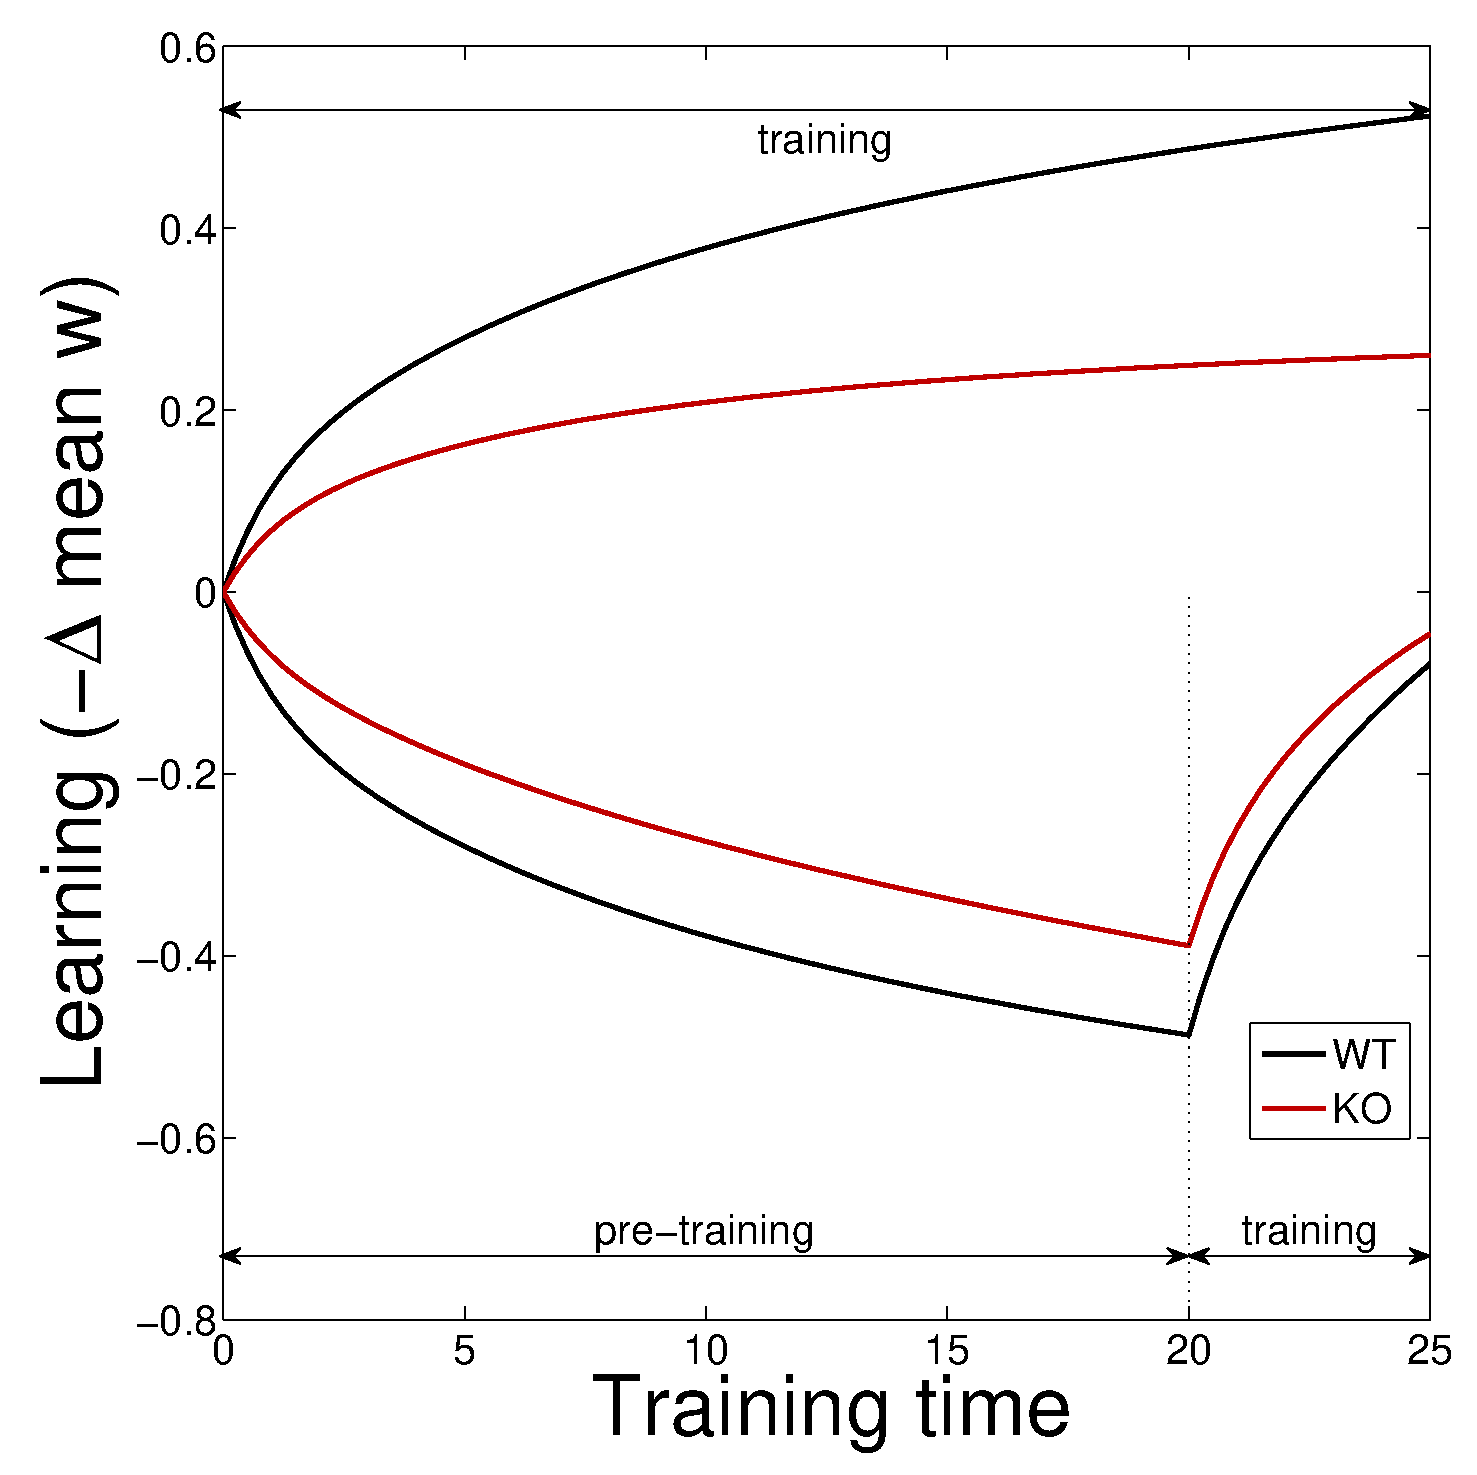
\includegraphics[width=7cm]{cascade_short_learn.eps}}\label{fig:cascade_short_learn}
  \item\aligntop{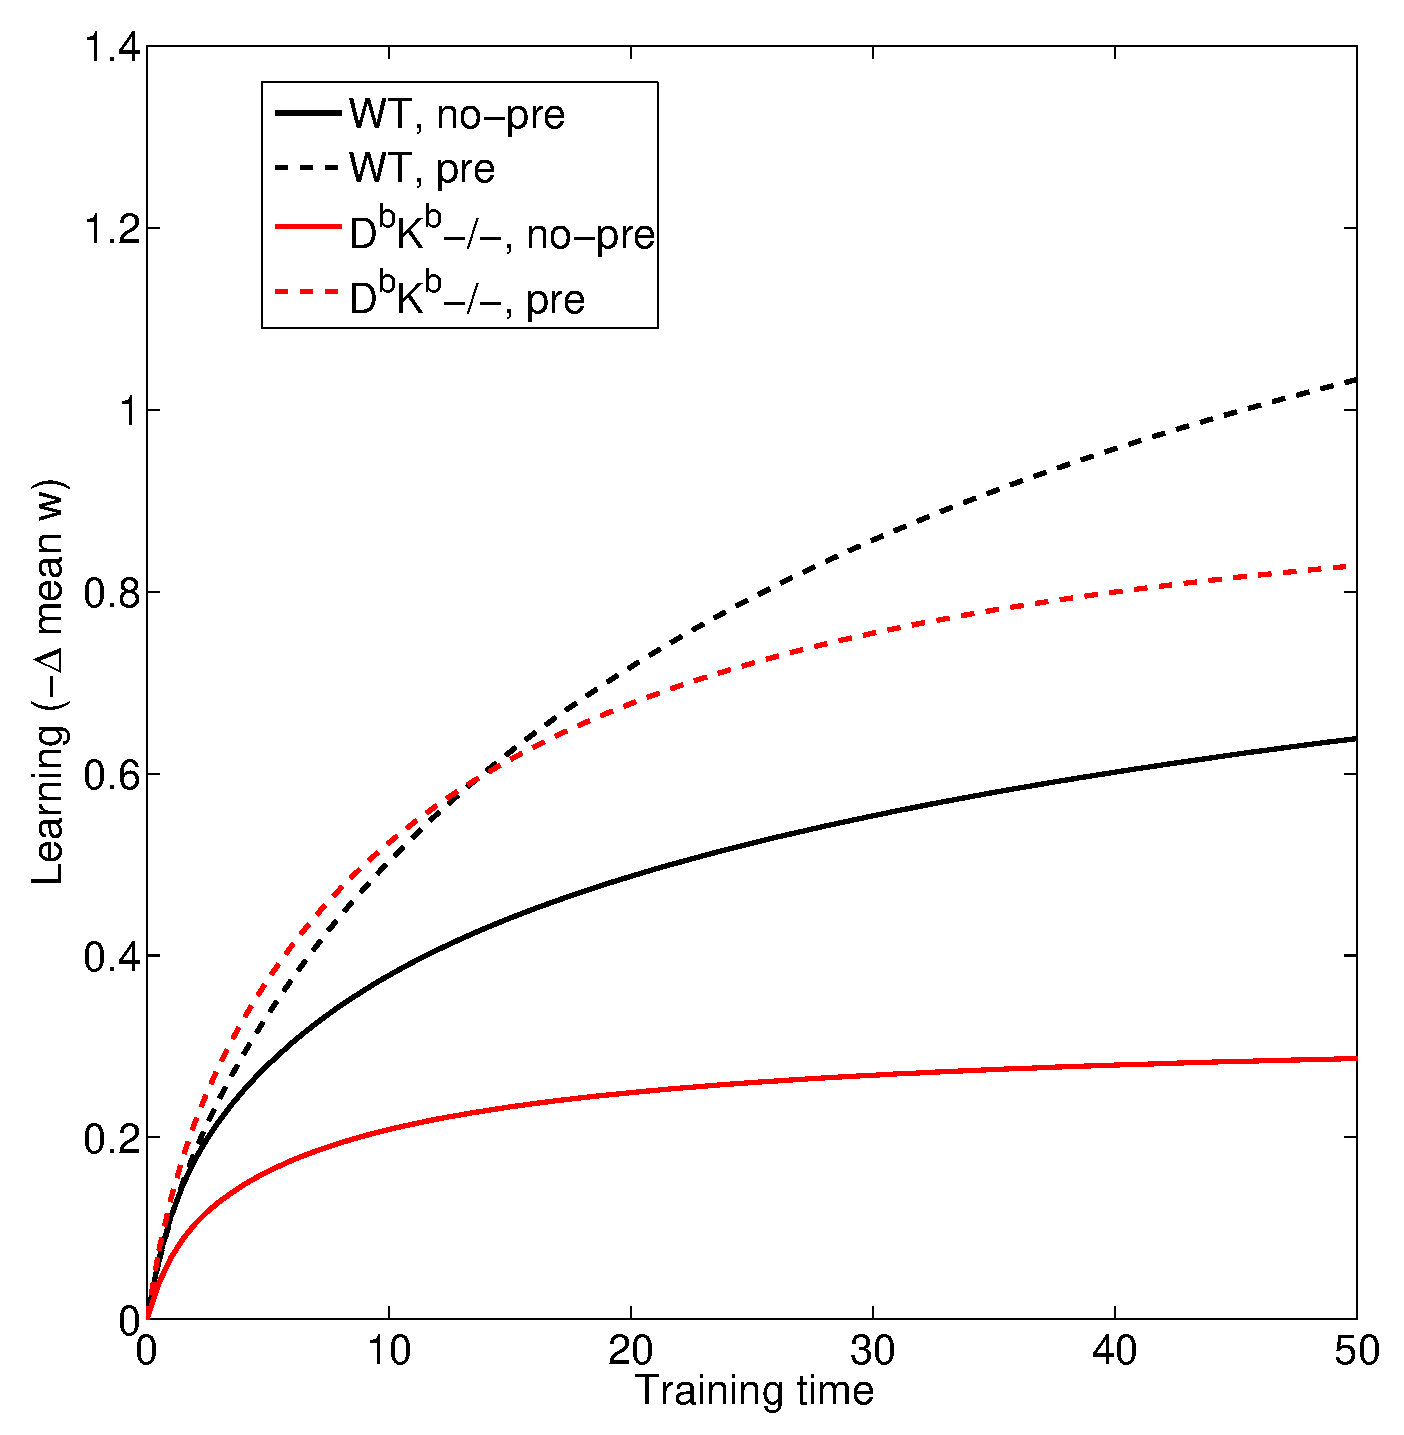
\includegraphics[width=7cm]{cascade_short_learnS.eps}}\label{fig:cascade_short_learnS}
  \item\label{fig:cascade_short_eq}\begin{myenumi}
                    \item\aligntop{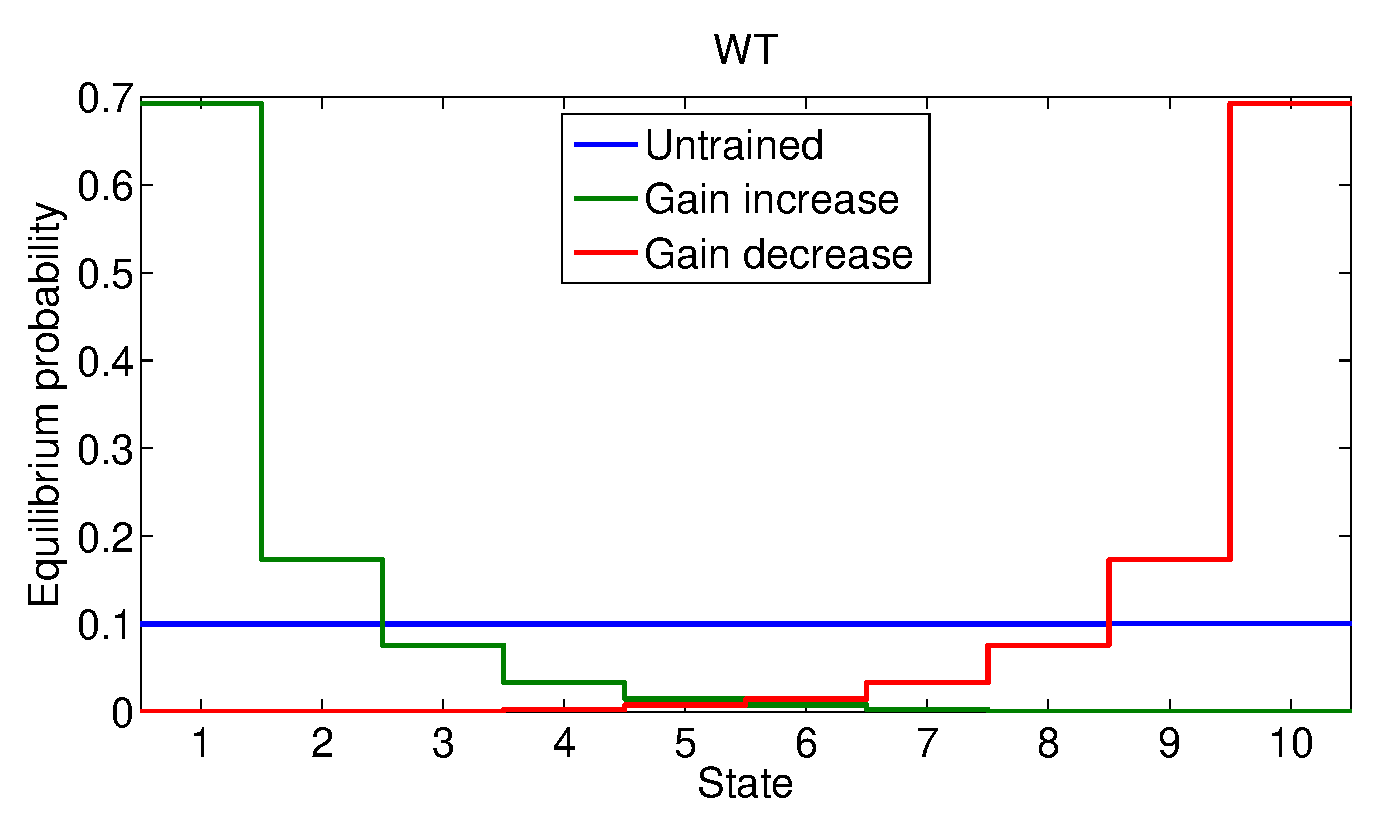
\includegraphics[width=7cm]{cascade_short_eq_WT.eps}}\label{fig:cascade_short_eq_WT}
                    \item\aligntop{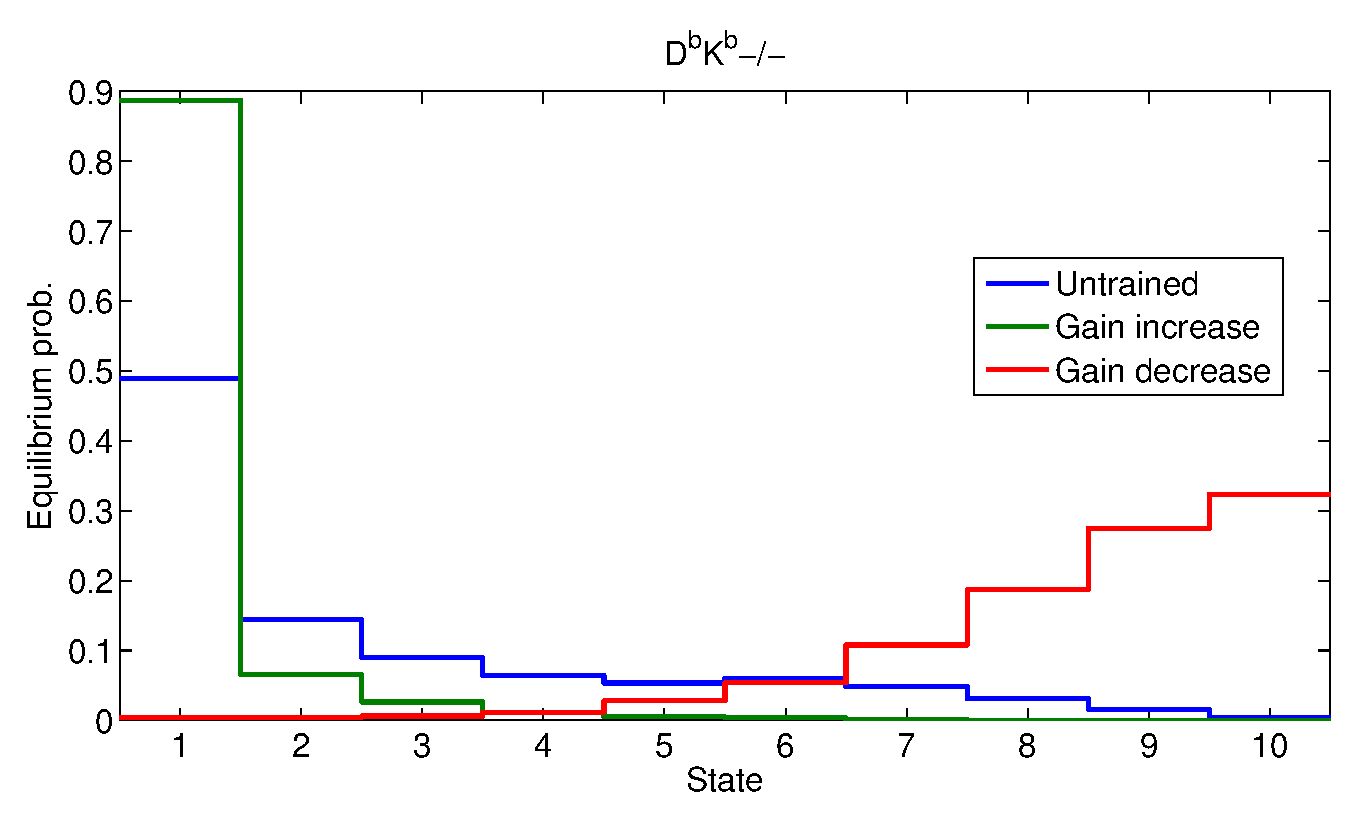
\includegraphics[width=7cm]{cascade_short_eq_KO.eps}}\label{fig:cascade_short_eq_KO}
                  \end{myenumi}
  \item\label{fig:cascade_short_pr}\begin{myenumi}
                    \item\aligntop{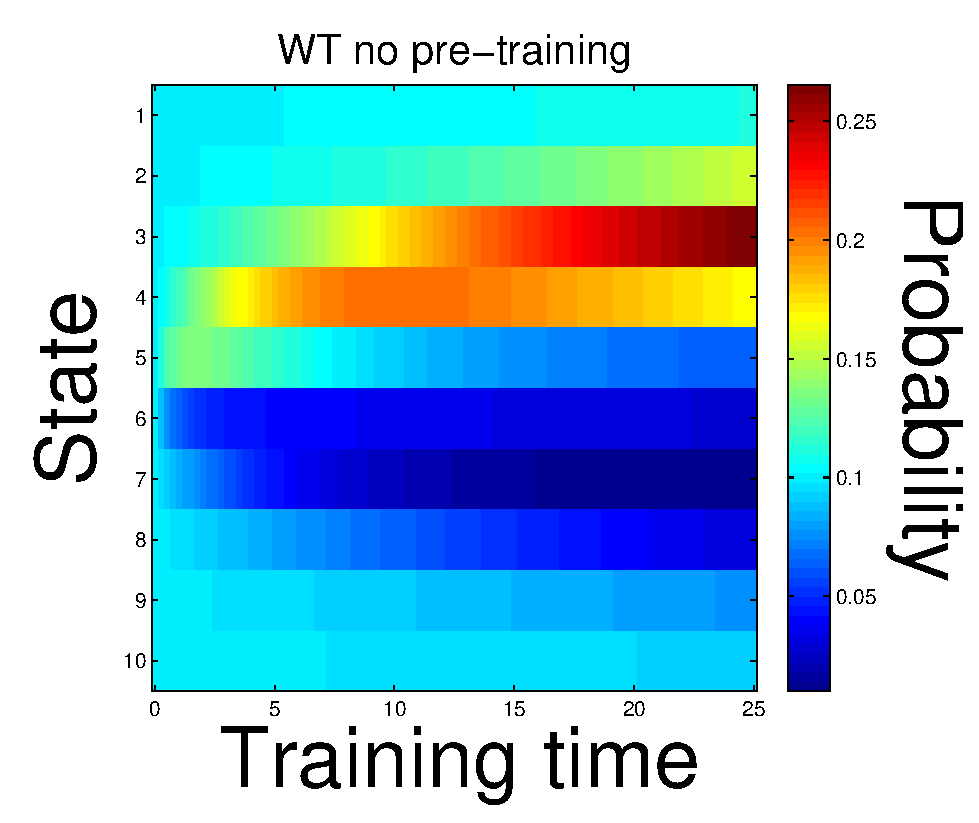
\includegraphics[width=3cm]{cascade_short_pr_WT_nopre.eps}}\label{fig:cascade_short_pr_WT_nopre}
                    \item\aligntop{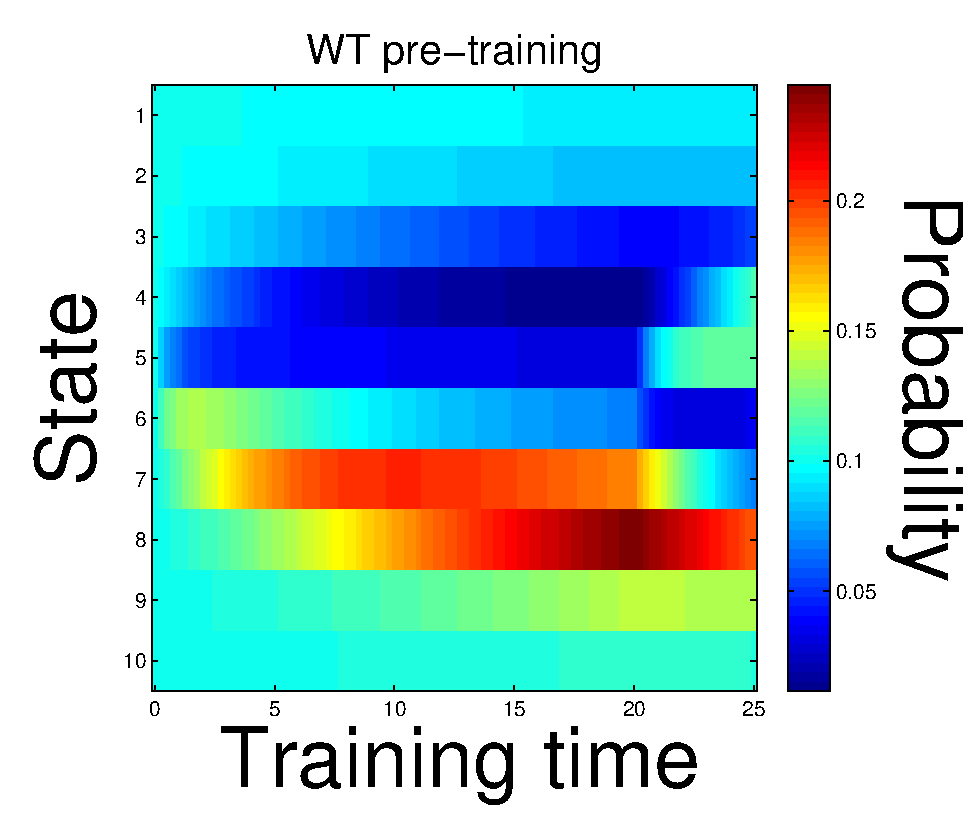
\includegraphics[width=3cm]{cascade_short_pr_WT_pre.eps}}\label{fig:cascade_short_pr_WT_pre}
                    \item\aligntop{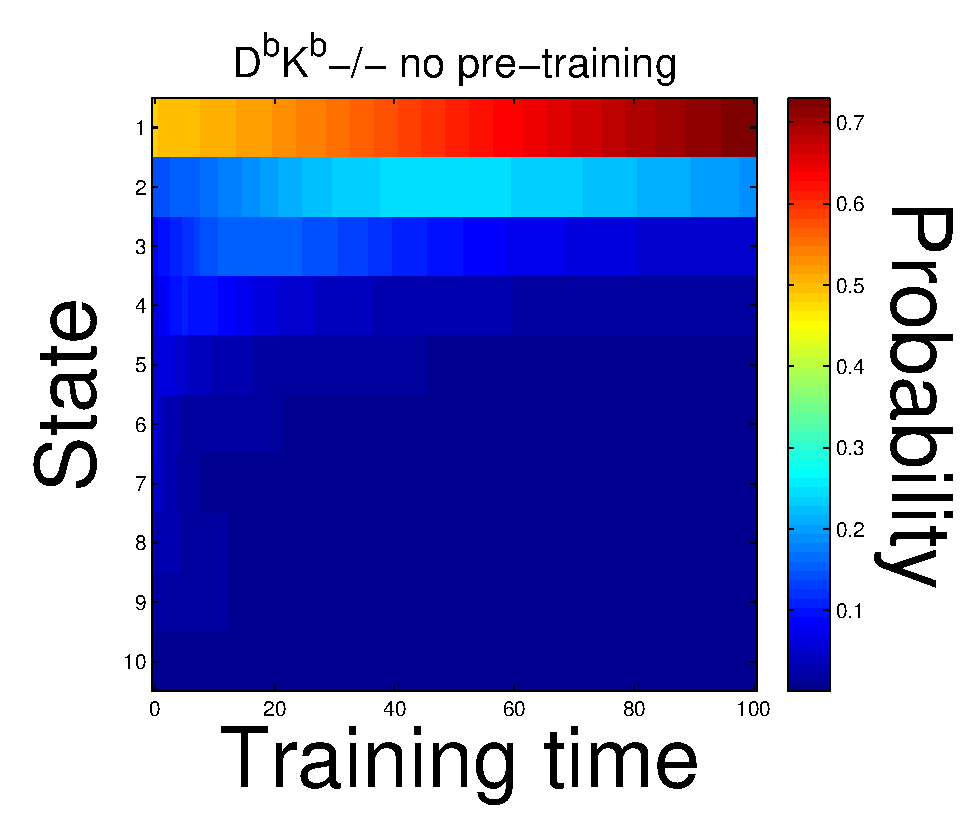
\includegraphics[width=3cm]{cascade_short_pr_KO_nopre.eps}}\label{fig:cascade_short_pr_KO_nopre}
                    \item\aligntop{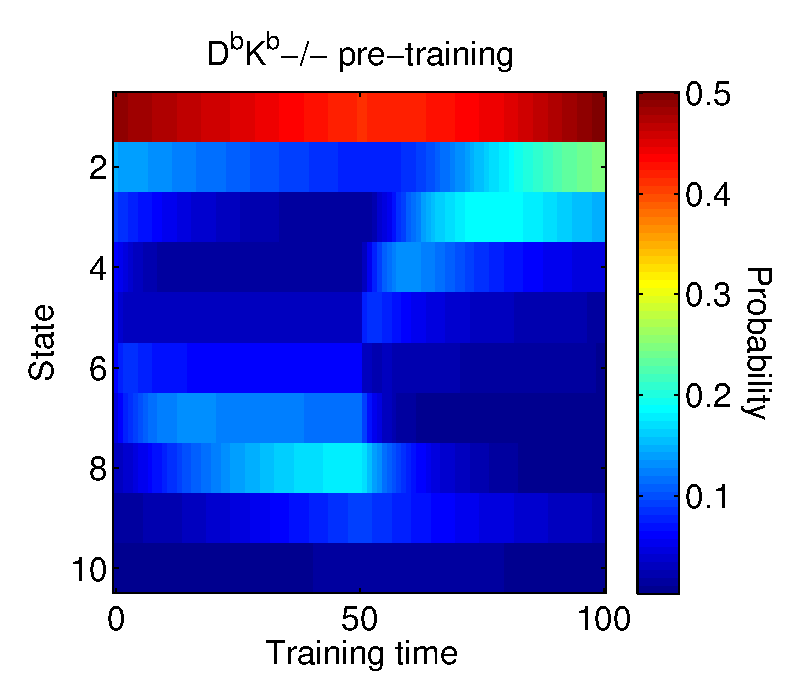
\includegraphics[width=3cm]{cascade_short_pr_KO_pre.eps}}\label{fig:cascade_short_pr_KO_pre}
                  \end{myenumi}
 \end{myenuma}
 \end{center}
  \caption{Simulation results for cascade model with short pre-training ($rt_\text{pre}=50$).
  Other parameters can be found in \autoref{tab:params}.
  (\ref{fig:cascade_short_learn}) Learning curves for wild-type and \KO\ mutant with and without pre-training.
  (\ref{fig:cascade_short_learnS}) Learning curves restricted to gain-increase training.
  (\ref{fig:cascade_short_eq}) Equilibrium distributions without training or with gain-increase/decrease training for (\ref{fig:cascade_short_eq_WT}) wild-type and (\ref{fig:cascade_short_eq_KO}) \KO\ mutant.
  (\ref{fig:cascade_short_pr}) Evolution of probability distributions for (\ref{fig:cascade_short_pr_WT_nopre}\ref{fig:cascade_short_pr_WT_pre}) wild-type and  (\ref{fig:cascade_short_pr_KO_nopre}\ref{fig:cascade_short_pr_KO_pre}) \KO\ mutant without (\ref{fig:cascade_short_pr_WT_nopre},\ref{fig:cascade_short_pr_KO_nopre}) and with (\ref{fig:cascade_short_pr_WT_pre},\ref{fig:cascade_short_pr_KO_pre}) pre-training. } \label{fig:cascade_short}
\end{figure}


\begin{figure}
 \begin{center}
 \begin{myenuma}
  \item\aligntop{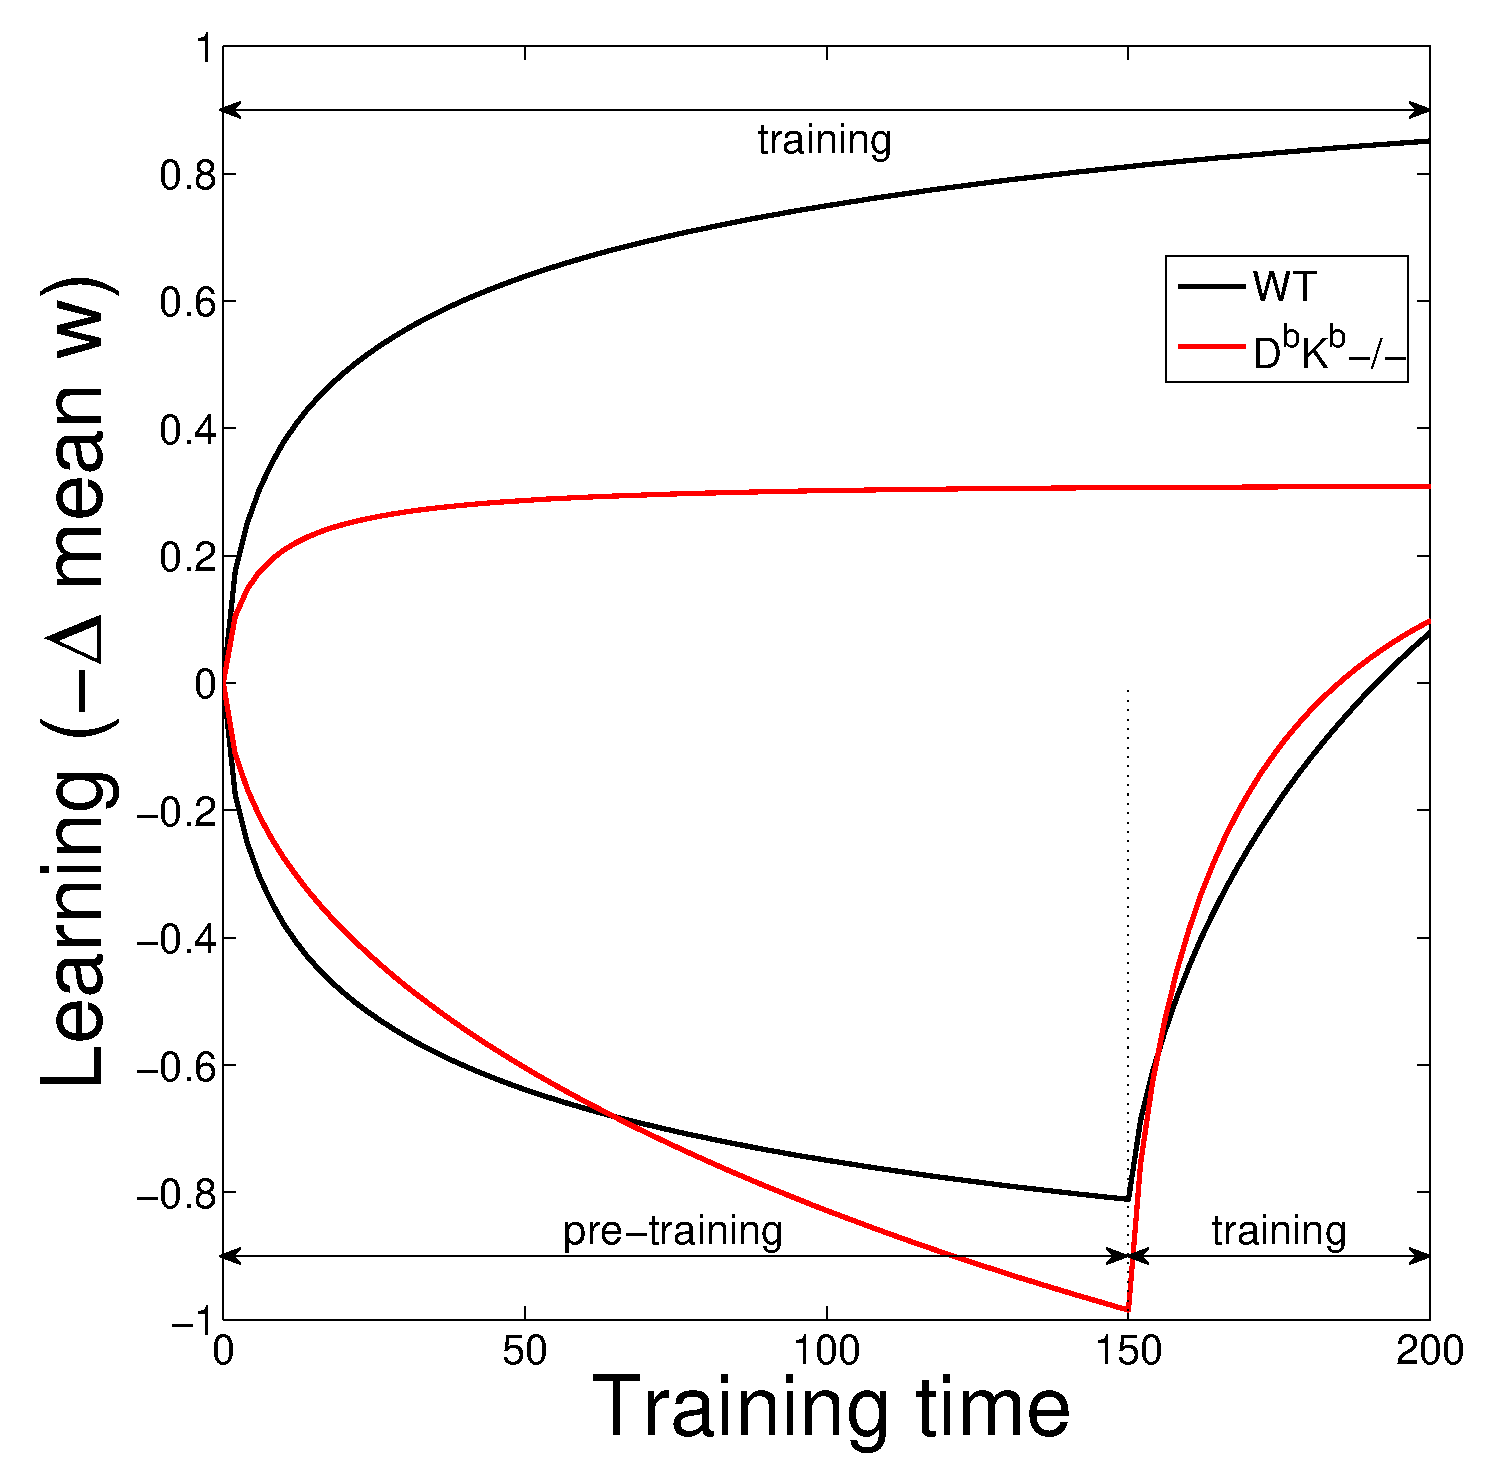
\includegraphics[width=7cm]{cascade_long_learn.eps}}\label{fig:cascade_long_learn}
  \item\aligntop{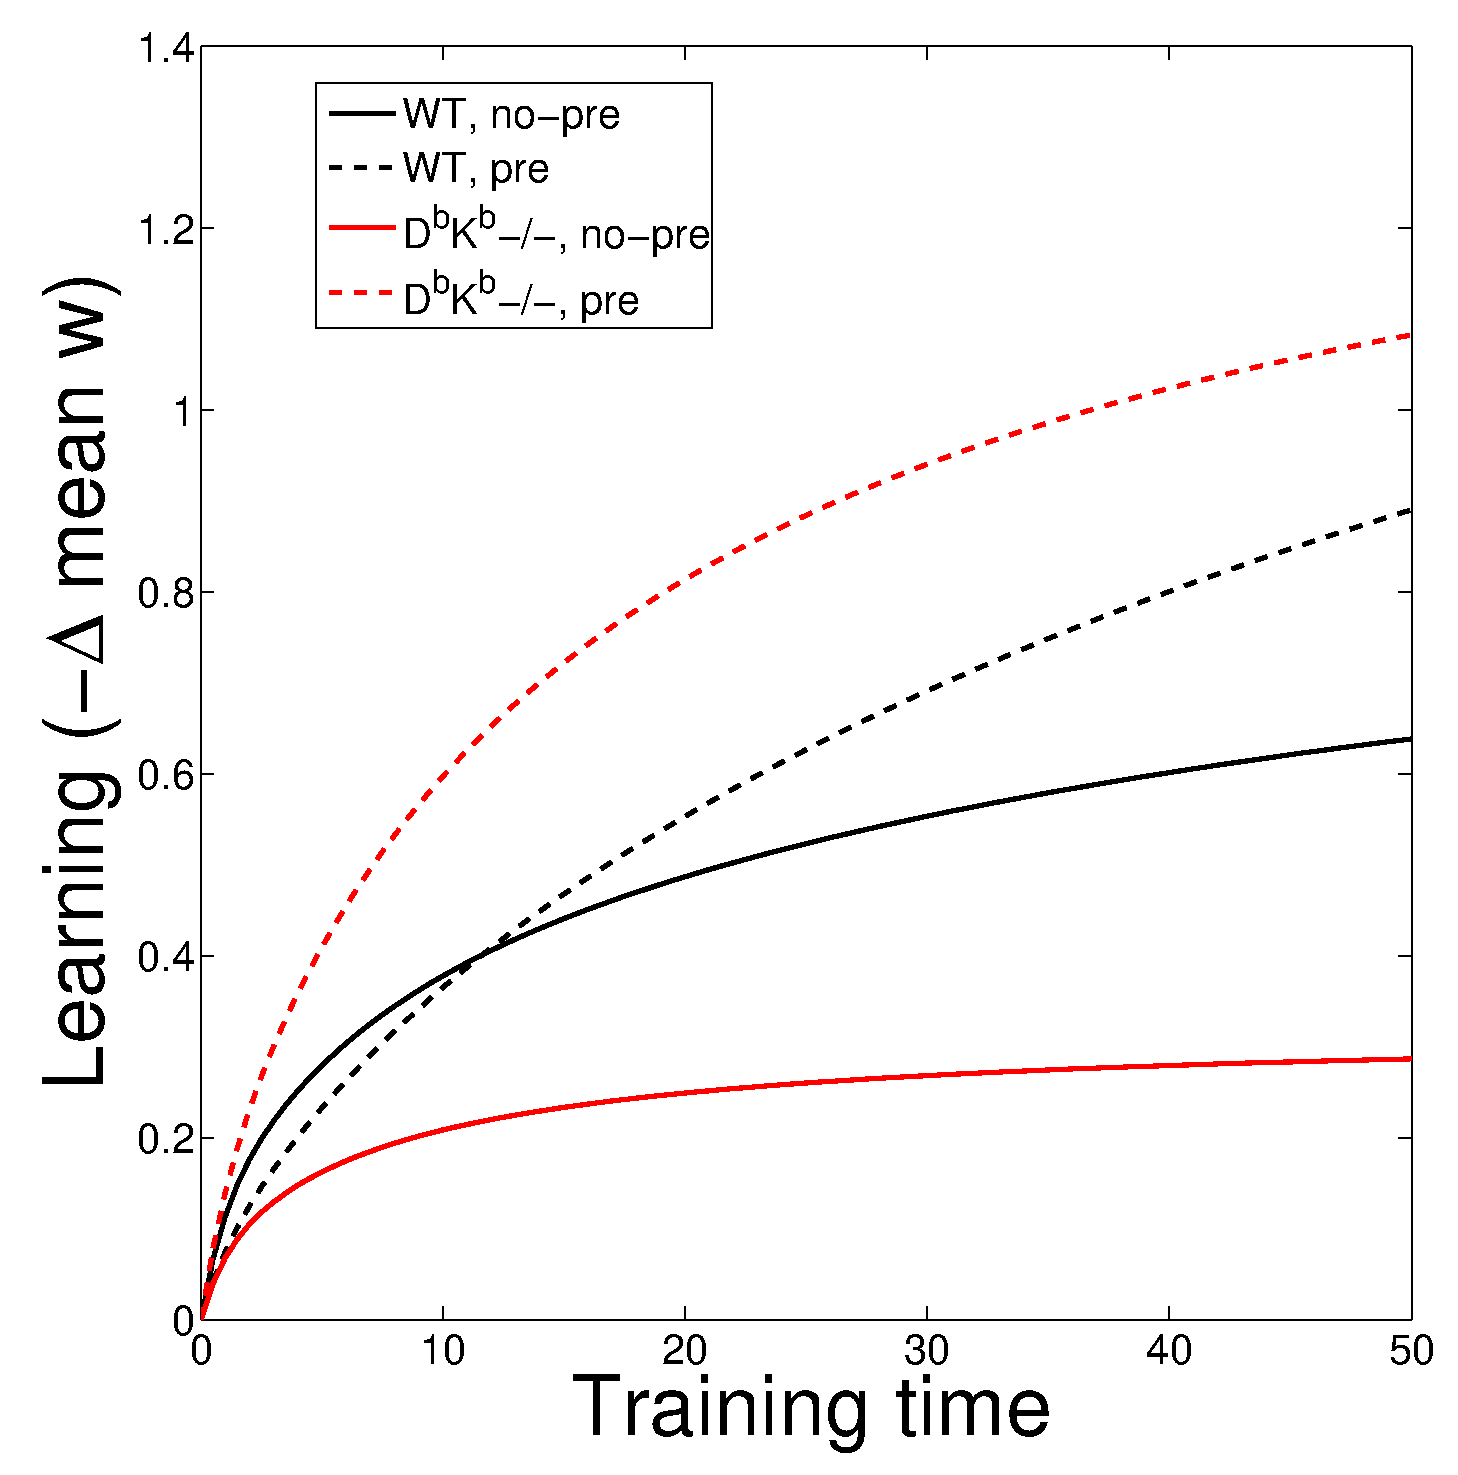
\includegraphics[width=7cm]{cascade_long_learnS.eps}}\label{fig:cascade_long_learnS}
  \item\label{fig:cascade_long_eq}\begin{myenumi}
                    \item\aligntop{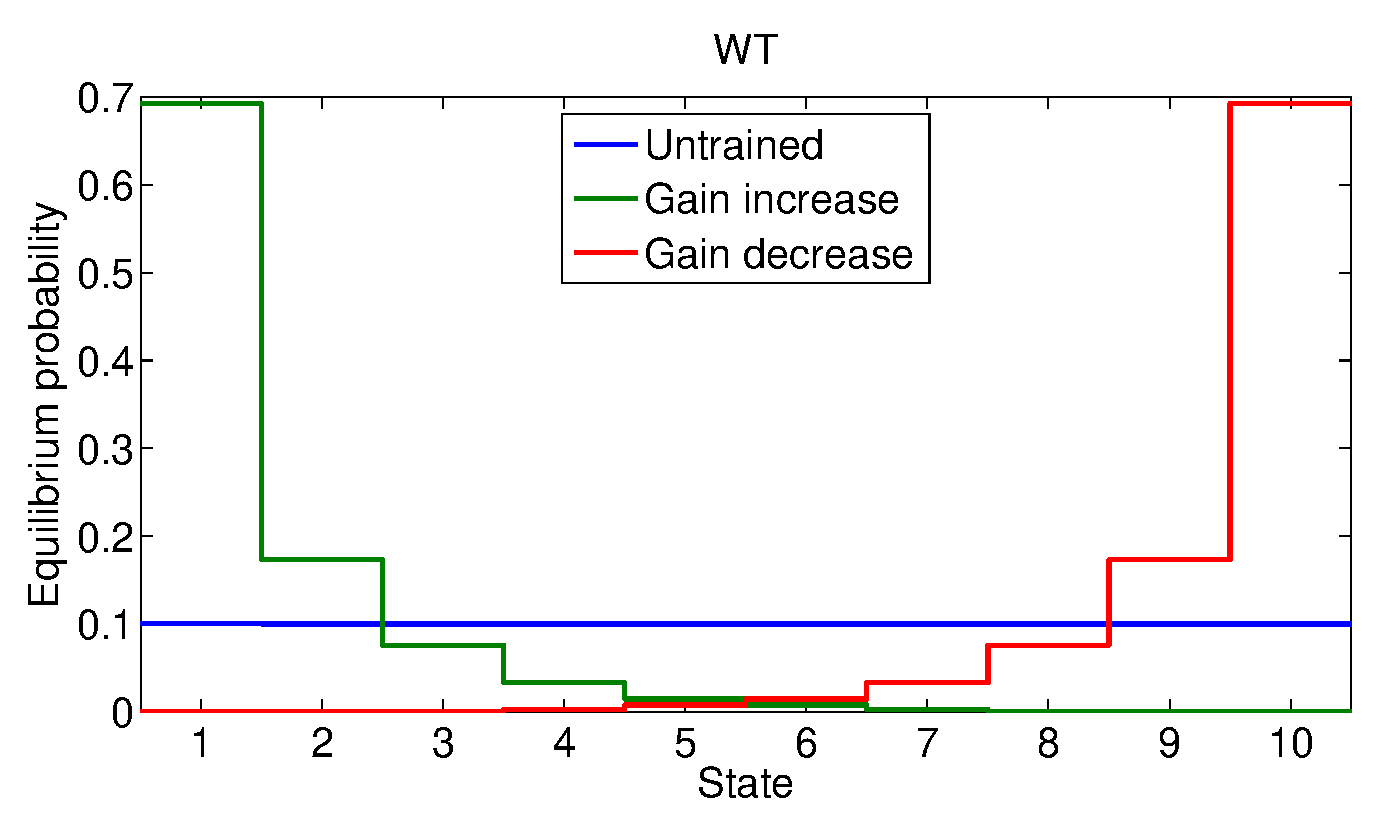
\includegraphics[width=7cm]{cascade_long_eq_WT.eps}}\label{fig:cascade_long_eq_WT}
                    \item\aligntop{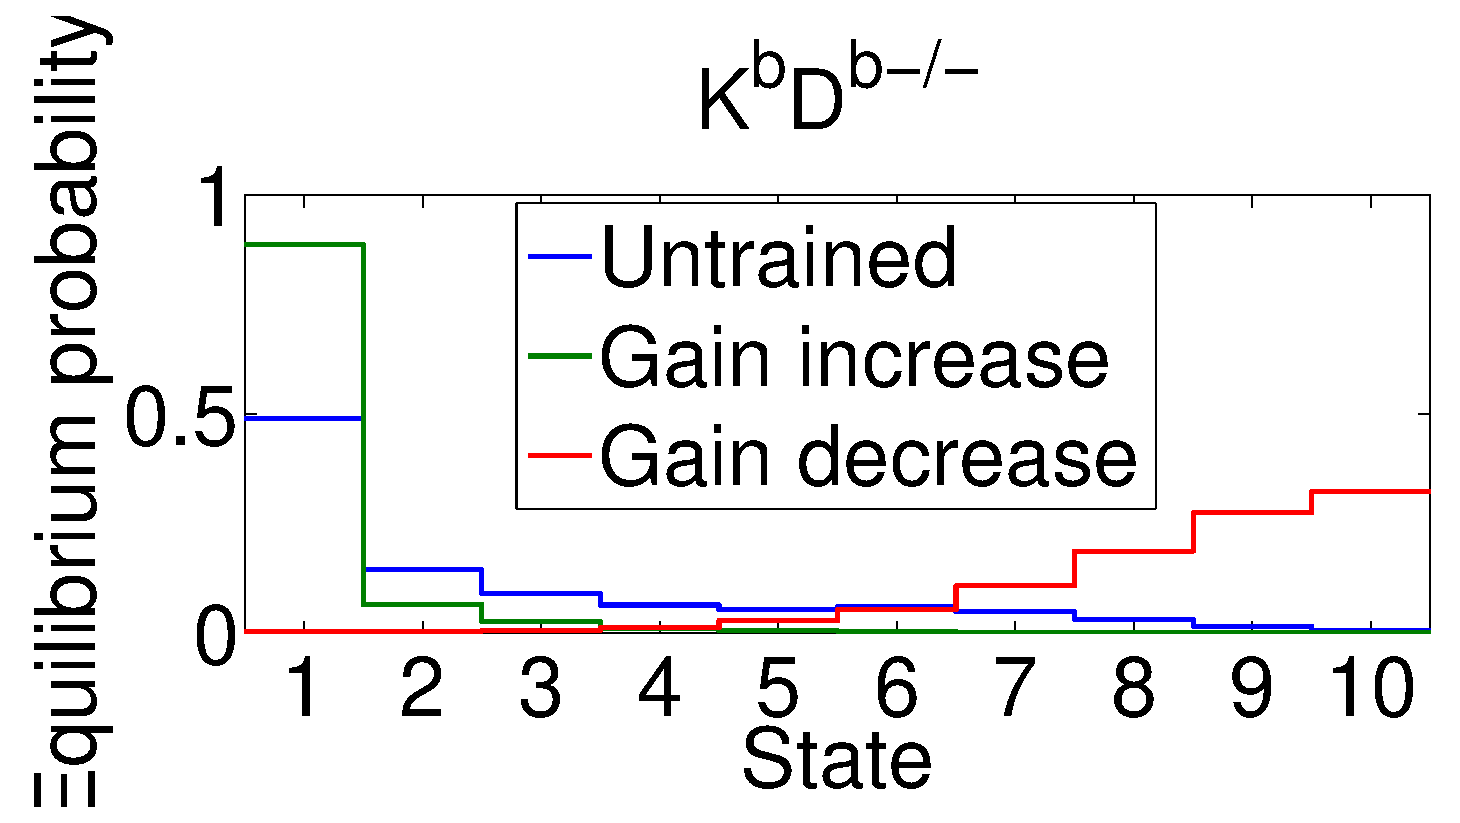
\includegraphics[width=7cm]{cascade_long_eq_KO.eps}}\label{fig:cascade_long_eq_KO}
                  \end{myenumi}
  \item\label{fig:cascade_long_pr}\begin{myenumi}
                    \item\aligntop{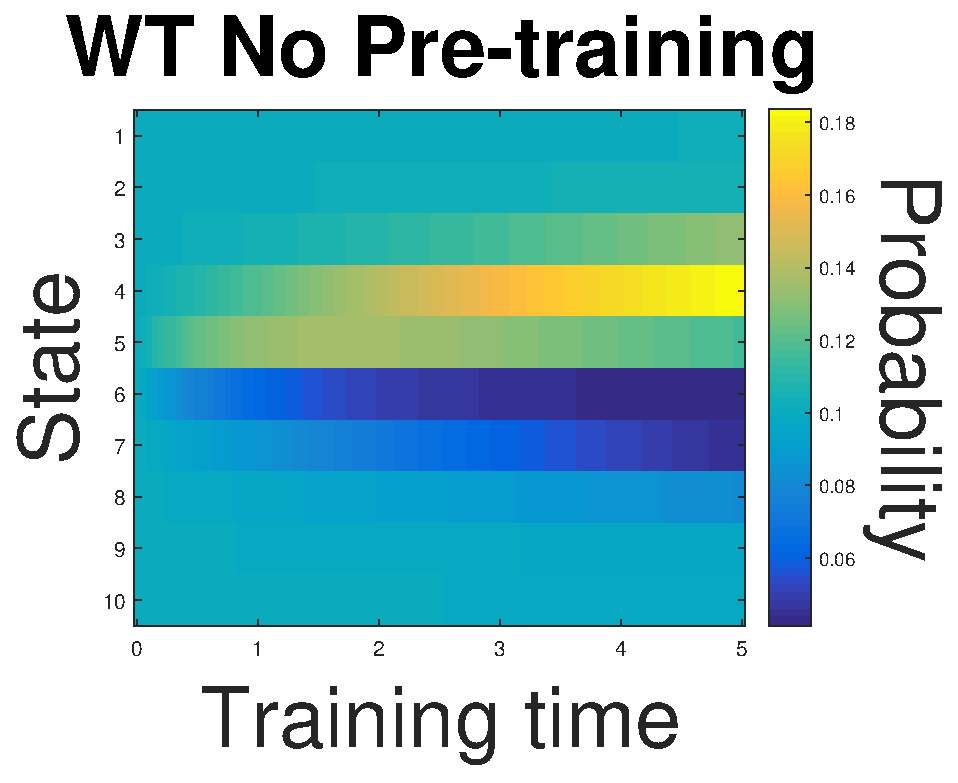
\includegraphics[width=3cm]{cascade_long_pr_WT_nopre.eps}}\label{fig:cascade_long_pr_WT_nopre}
                    \item\aligntop{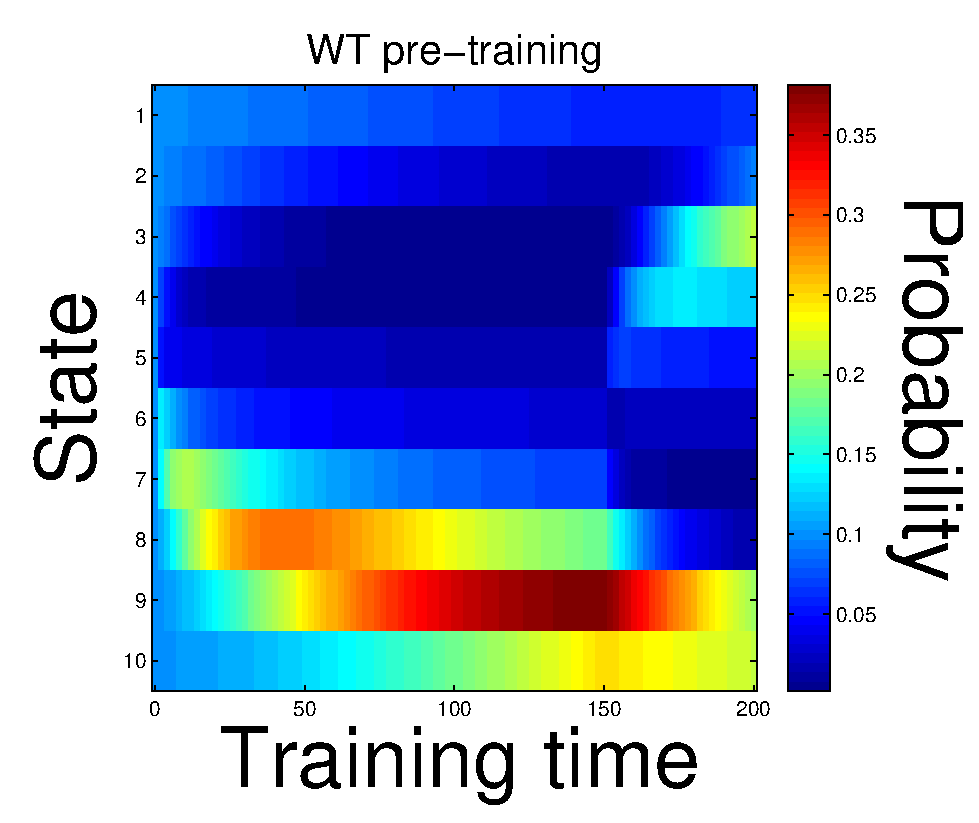
\includegraphics[width=3cm]{cascade_long_pr_WT_pre.eps}}\label{fig:cascade_long_pr_WT_pre}
                    \item\aligntop{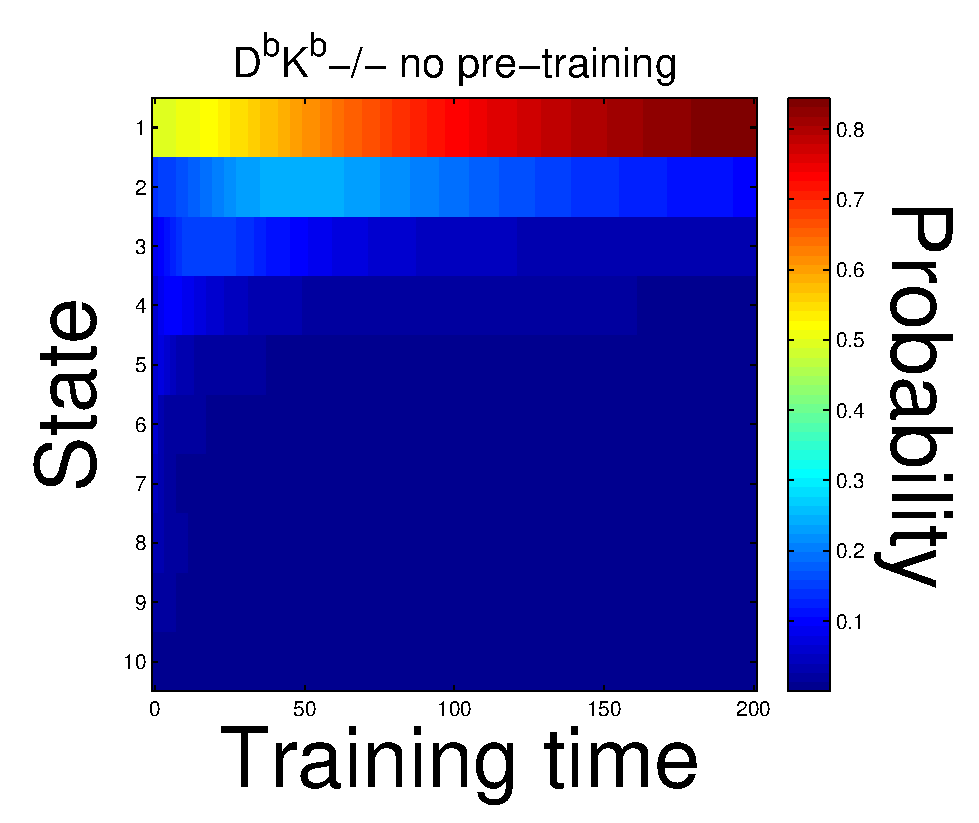
\includegraphics[width=3cm]{cascade_long_pr_KO_nopre.eps}}\label{fig:cascade_long_pr_KO_nopre}
                    \item\aligntop{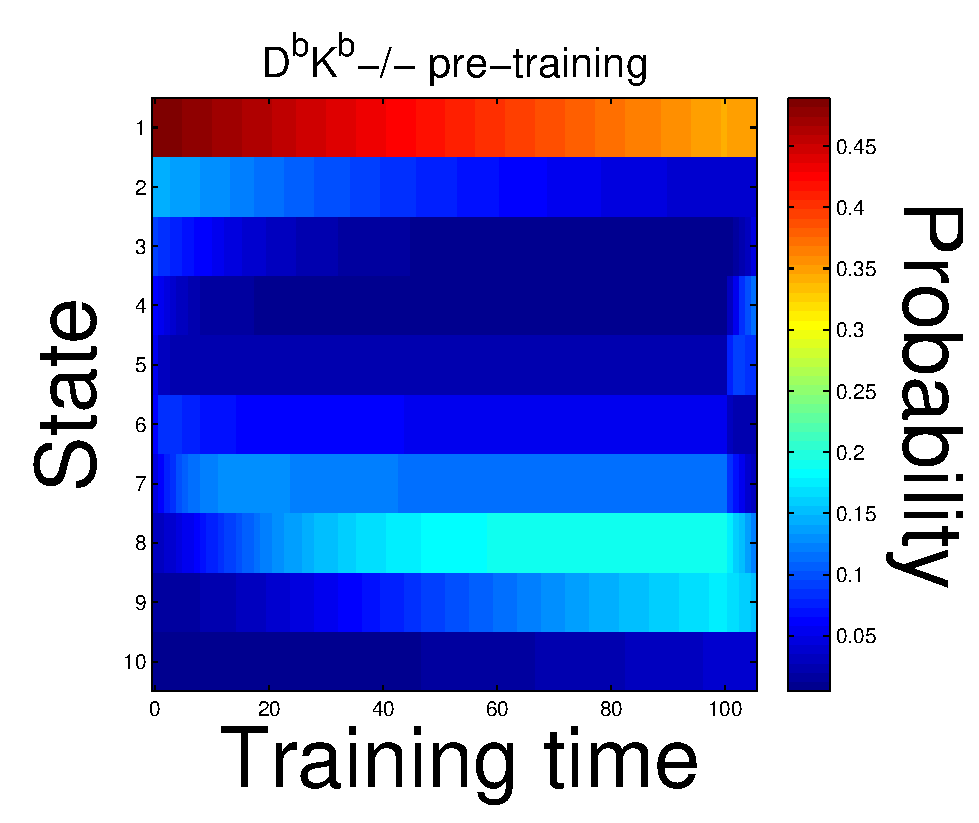
\includegraphics[width=3cm]{cascade_long_pr_KO_pre.eps}}\label{fig:cascade_long_pr_KO_pre}
                  \end{myenumi}
 \end{myenuma}
 \end{center}
  \caption{Simulation results for cascade model with long pre-training ($rt_\text{pre}=150$).
  Other parameters can be found in \autoref{tab:params}.
  (\ref{fig:cascade_long_learn}) Learning curves for wild-type and \KO\ mutant with and without pre-training.
  (\ref{fig:cascade_long_learnS}) Learning curves restricted to gain-increase training.
  (\ref{fig:cascade_long_eq}) Equilibrium distributions without training or with gain-increase/decrease training for (\ref{fig:cascade_long_eq_WT}) wild-type and (\ref{fig:cascade_long_eq_KO}) \KO\ mutant.
  (\ref{fig:cascade_long_pr}) Evolution of probability distributions for (\ref{fig:cascade_long_pr_WT_nopre}\ref{fig:cascade_long_pr_WT_pre}) wild-type and  (\ref{fig:cascade_long_pr_KO_nopre}\ref{fig:cascade_long_pr_KO_pre}) \KO\ mutant without (\ref{fig:cascade_long_pr_WT_nopre},\ref{fig:cascade_long_pr_KO_nopre}) and with (\ref{fig:cascade_long_pr_WT_pre},\ref{fig:cascade_long_pr_KO_pre}) pre-training. } \label{fig:cascade_long}
\end{figure}

The results of simulations of the cascade model can be seen in \autoref{fig:cascade_short} and \autoref{fig:cascade_long}.

In both of these, we see that the mutant is slower than wild-type without pre-training but faster with it.
This seems to be due to the fact that, without pre-training, very few synapses will be available for depression as most of them are already depressed (\autoref{fig:cascade_short}\ref{fig:cascade_short_eq}\ref{fig:cascade_short_eq_KO} and \ref{fig:cascade_short_pr}\ref{fig:cascade_short_pr_KO_nopre}).
With pre-training, some of them will now be potentiated (\autoref{fig:cascade_short}\ref{fig:cascade_short_eq}\ref{fig:cascade_short_eq_KO} and \ref{fig:cascade_short_pr}\ref{fig:cascade_short_pr_KO_pre}), and the enhanced depression can speed up learning.

With shorter pre-training, we see that it speeds up learning in both wild-type and mutant (see \autoref{fig:cascade_short}\ref{fig:cascade_short_learnS}), whereas experimentally this only happens for the mutant.
This is due to the fact that pre-training results in more synapses being potentiated, and thus ready for depression, but does not push them far enough down the cascade for the lower transition probabilities to slow down learning.

We can see from \autoref{fig:cascade_long}\ref{fig:cascade_long_learnS} that longer pre-training pushes the synapses further down the cascade, slow in down learning for the wild-type.
This effect is weaker for the mutant, as the equilibrium distribution is not as heavily concentrated at the end (see \autoref{fig:cascade_long}\ref{fig:cascade_long_eq}\ref{fig:cascade_long_eq_KO}).


\subsubsection{Multistate model}\label{sec:multistate}

\begin{figure}
 \begin{center}
 \begin{myenuma}
  \item\aligntop{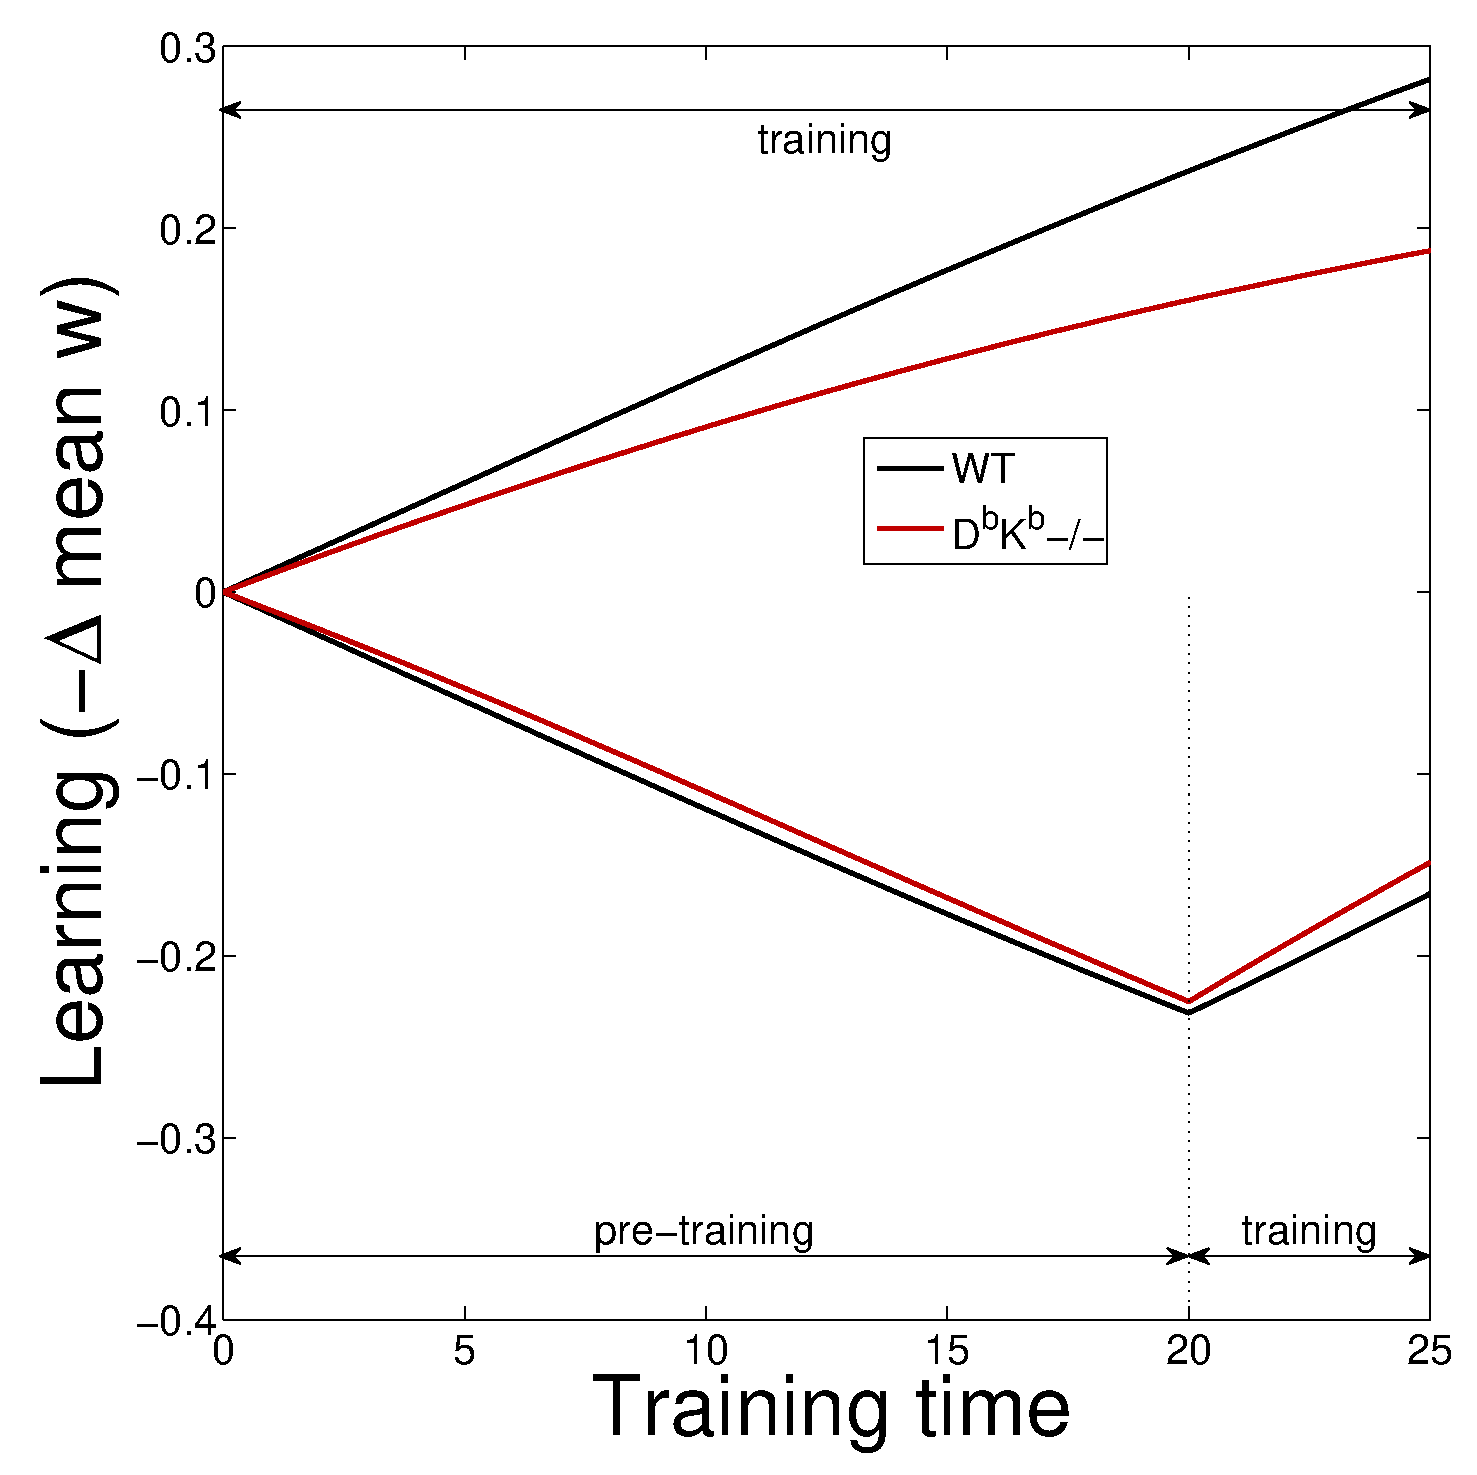
\includegraphics[width=7cm]{multistate_weak_learn.eps}}\label{fig:multistate_weak_learn}
  \item\aligntop{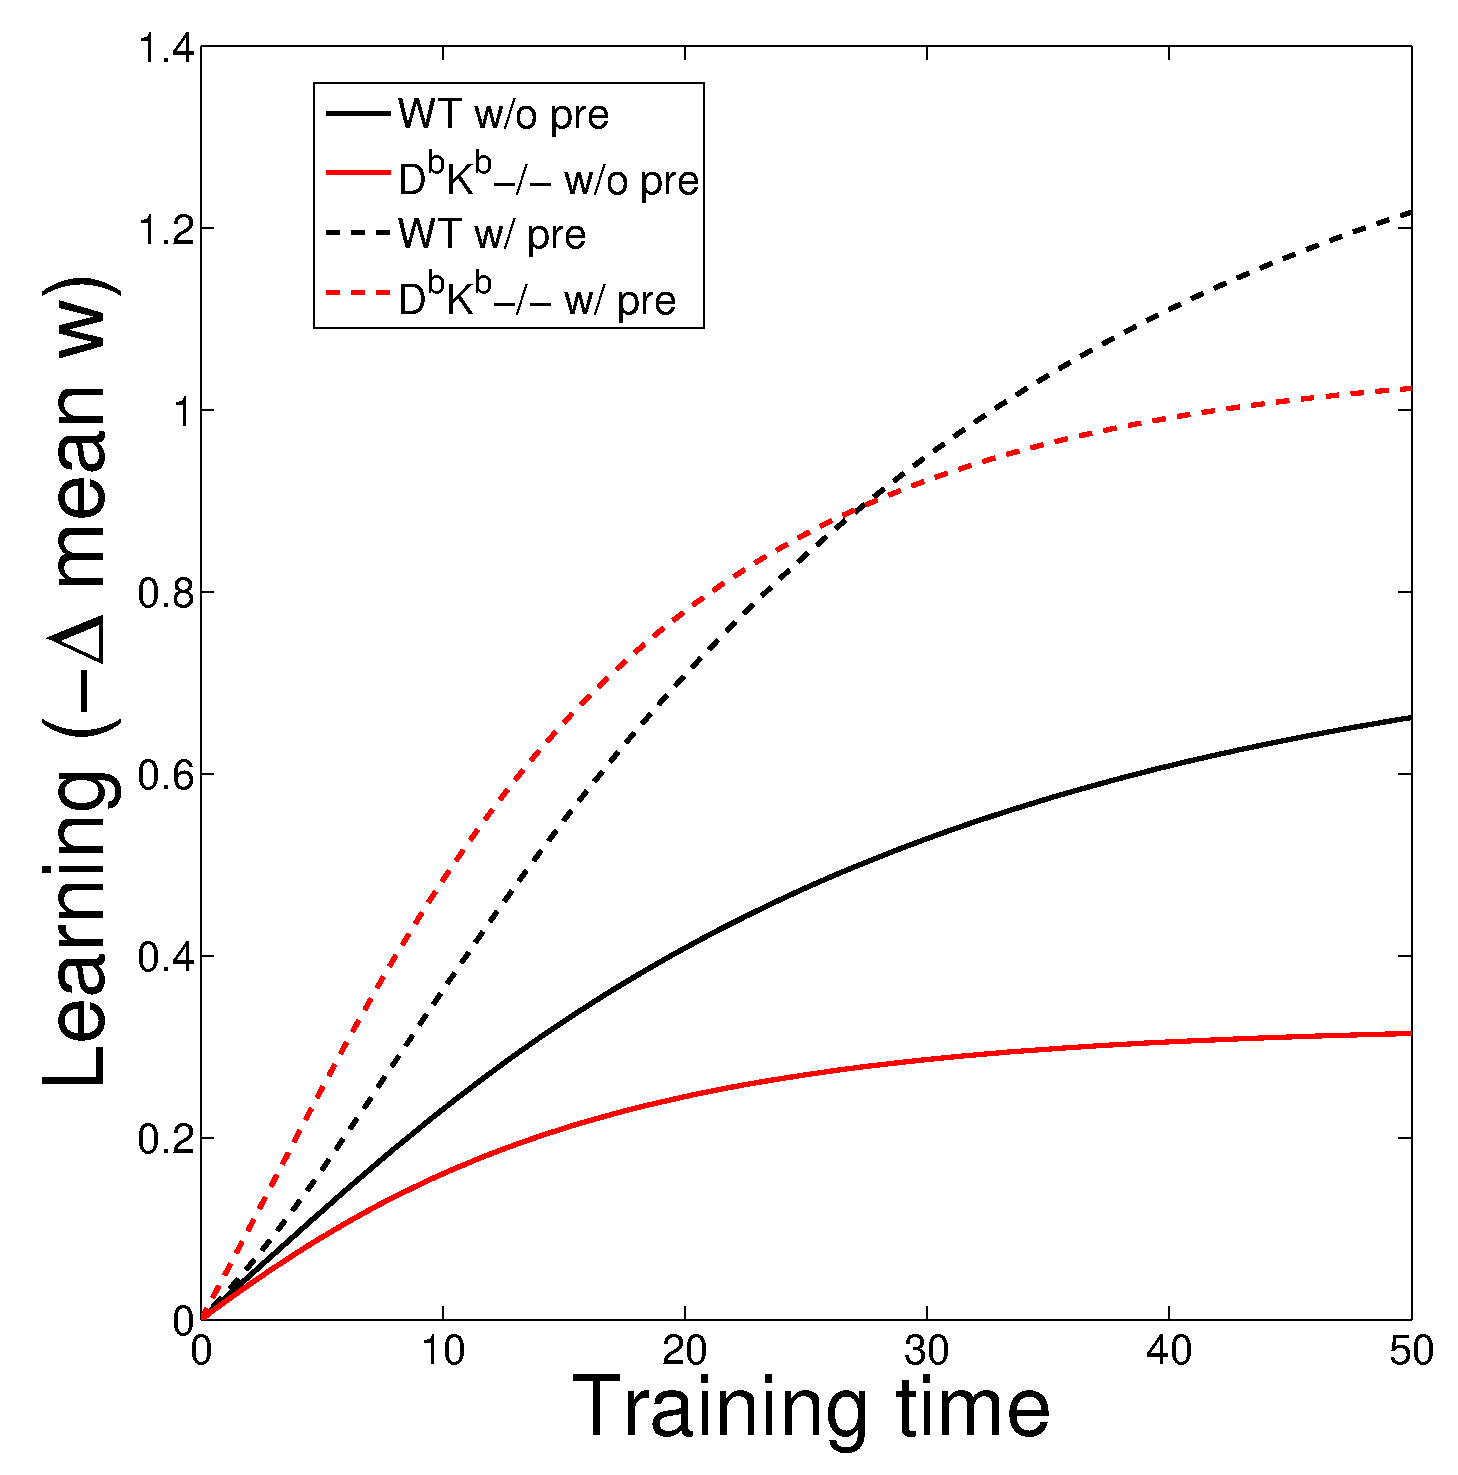
\includegraphics[width=7cm]{multistate_weak_learnS.eps}}\label{fig:multistate_weak_learnS}
  \item\label{fig:multistate_weak_eq}\begin{myenumi}
                    \item\aligntop{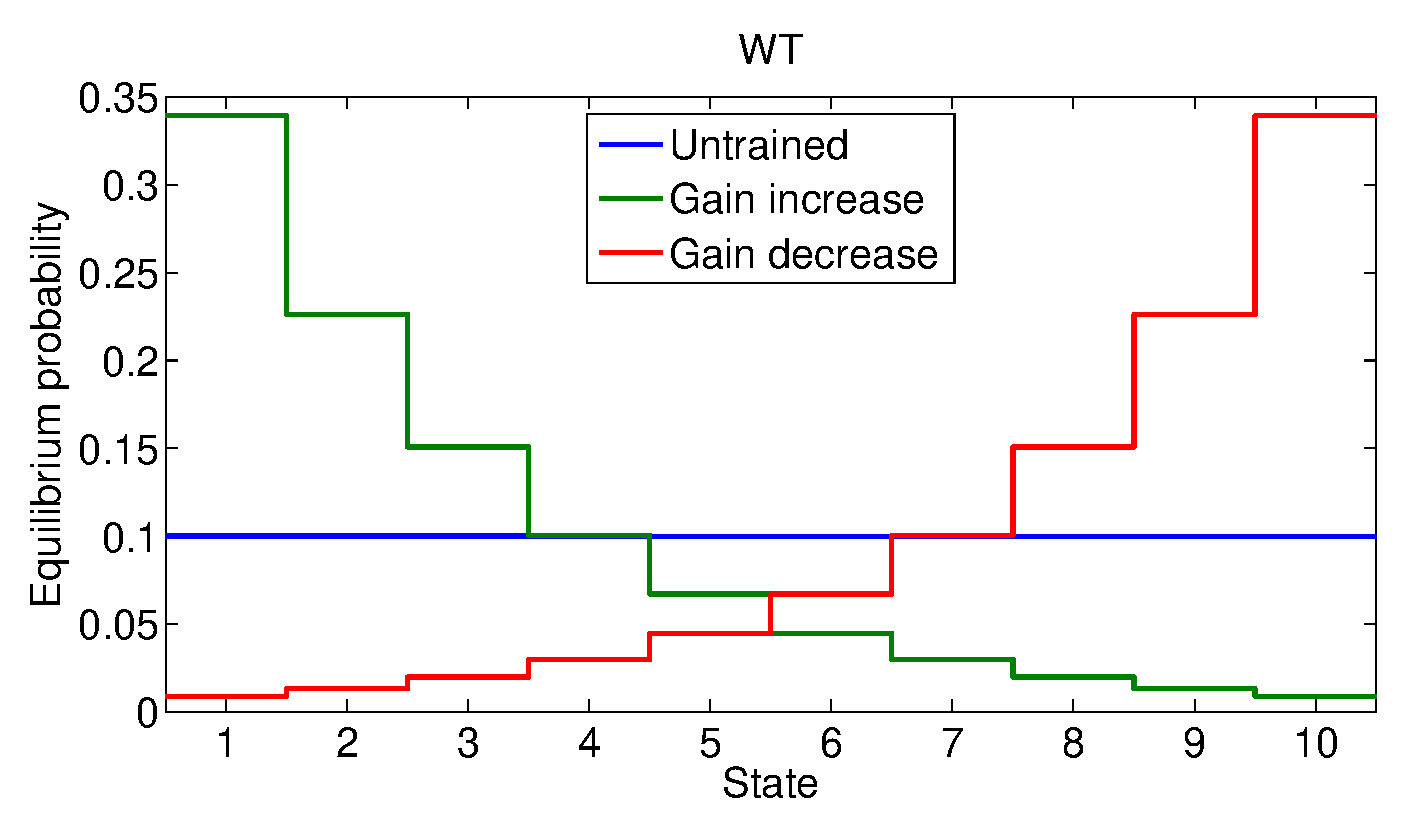
\includegraphics[width=7cm]{multistate_weak_eq_WT.eps}}\label{fig:multistate_weak_eq_WT}
                    \item\aligntop{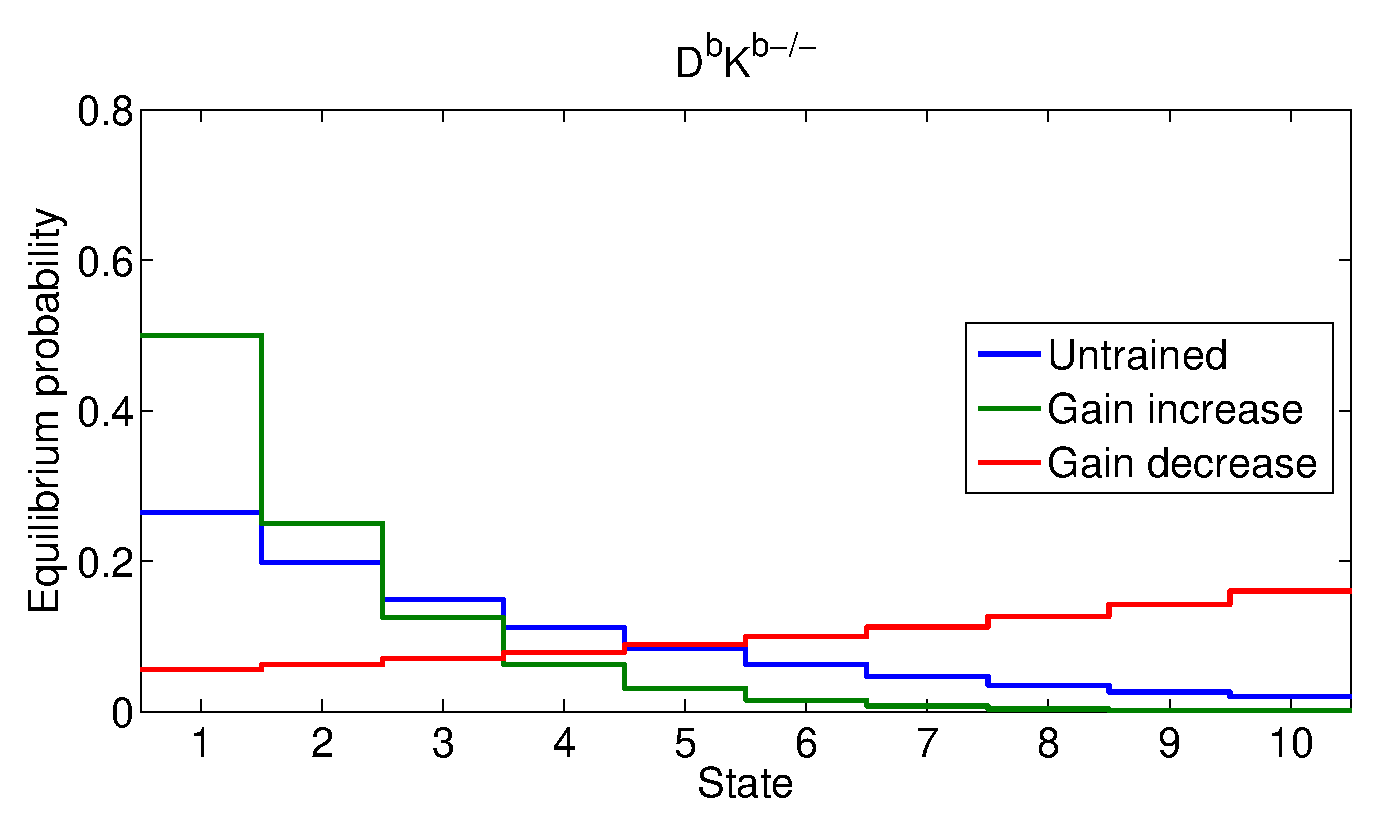
\includegraphics[width=7cm]{multistate_weak_eq_KO.eps}}\label{fig:multistate_weak_eq_KO}
                  \end{myenumi}
  \item\label{fig:multistate_weak_pr}\begin{myenumi}
                    \item\aligntop{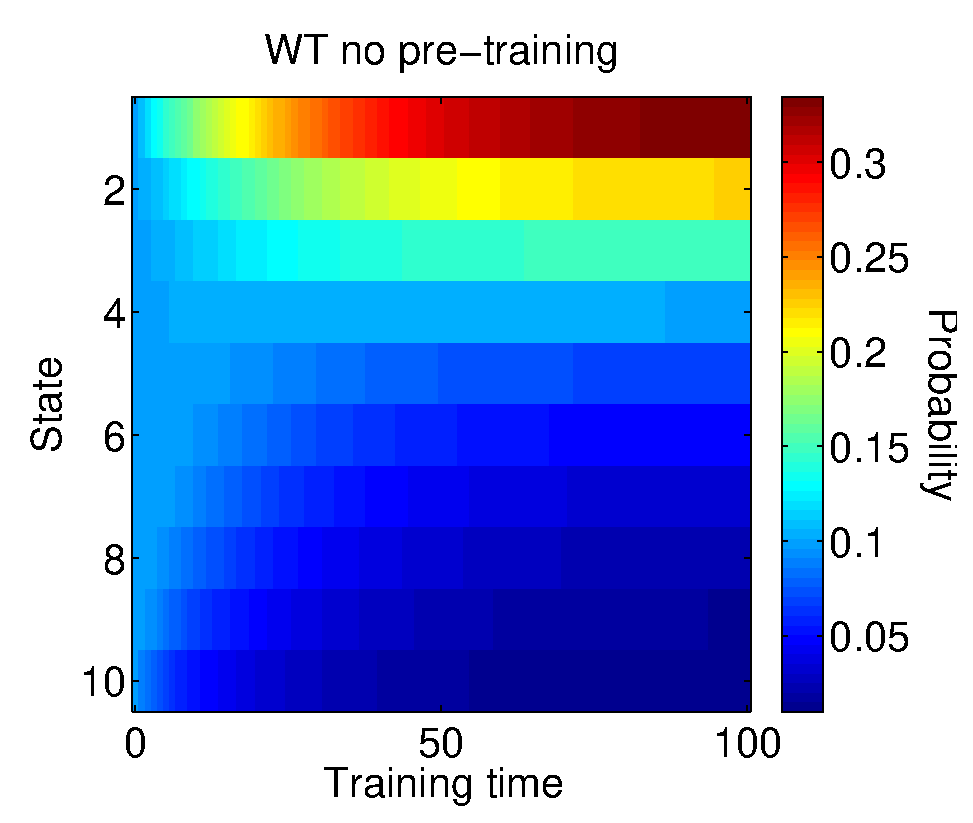
\includegraphics[width=3cm]{multistate_weak_pr_WT_nopre.eps}}\label{fig:multistate_weak_pr_WT_nopre}
                    \item\aligntop{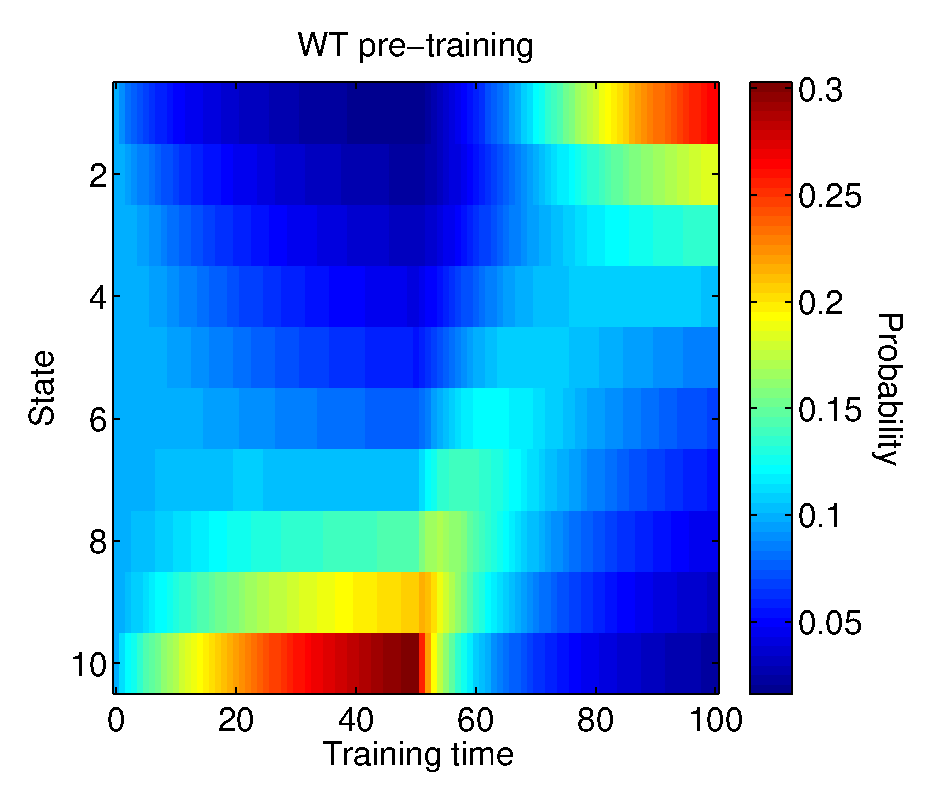
\includegraphics[width=3cm]{multistate_weak_pr_WT_pre.eps}}\label{fig:multistate_weak_pr_WT_pre}
                    \item\aligntop{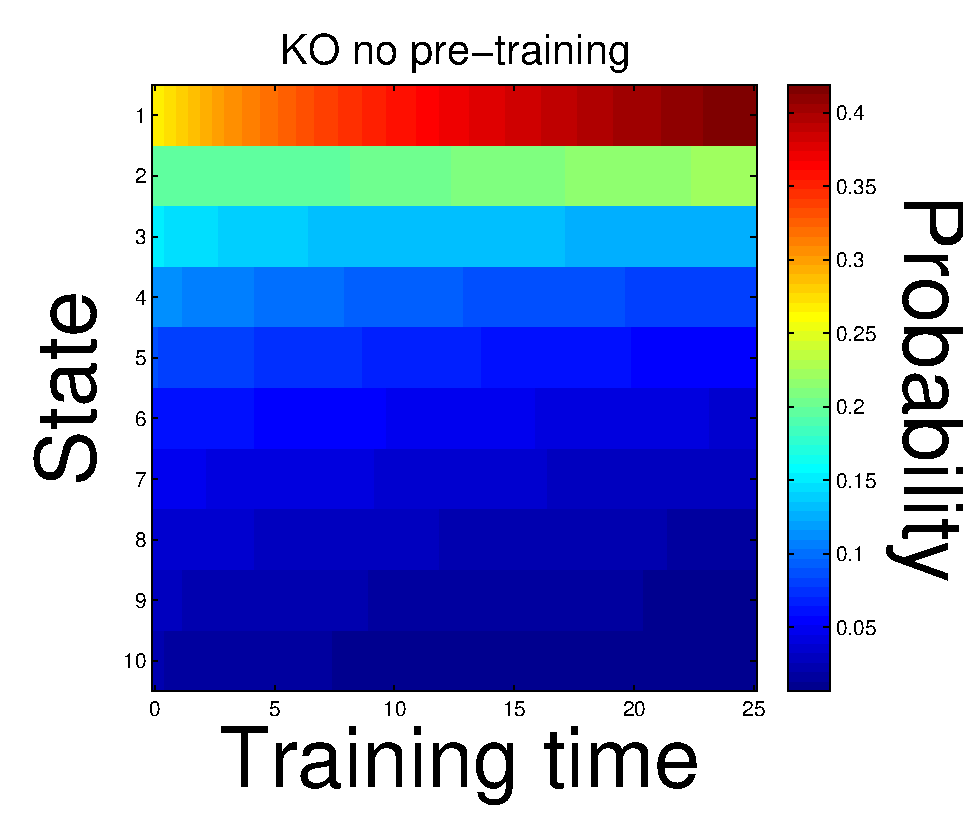
\includegraphics[width=3cm]{multistate_weak_pr_KO_nopre.eps}}\label{fig:multistate_weak_pr_KO_nopre}
                    \item\aligntop{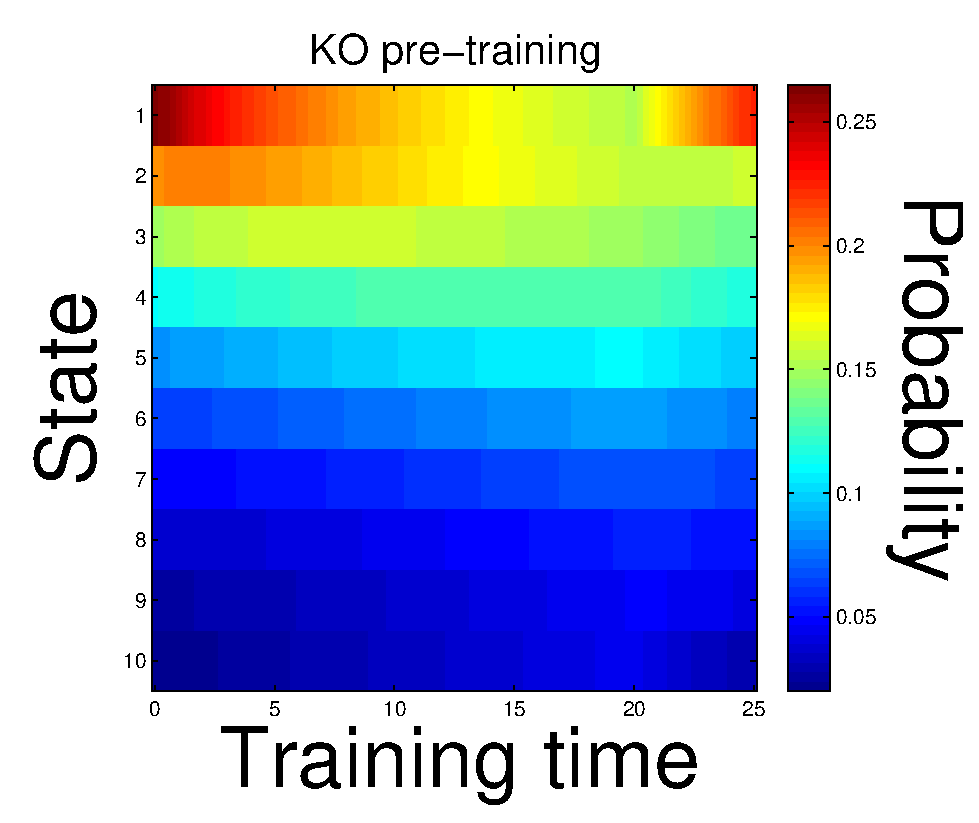
\includegraphics[width=3cm]{multistate_weak_pr_KO_pre.eps}}\label{fig:multistate_weak_pr_KO_pre}
                  \end{myenumi}
 \end{myenuma}
 \end{center}
  \caption{Simulation results for multistate model with weak training ($\Delta f=-0.1$).
  Other parameters can be found in \autoref{tab:params}.
  (\ref{fig:multistate_weak_learn}) Learning curves for wild-type and \KO\ mutant with and without pre-training.
  (\ref{fig:multistate_weak_learnS}) Learning curves restricted to gain-increase training.
  (\ref{fig:multistate_weak_eq}) Equilibrium distributions without training or with gain-increase/decrease training for (\ref{fig:multistate_weak_eq_WT}) wild-type and (\ref{fig:multistate_weak_eq_KO}) \KO\ mutant.
  (\ref{fig:multistate_weak_pr}) Evolution of probability distributions for (\ref{fig:multistate_weak_pr_WT_nopre}\ref{fig:multistate_weak_pr_WT_pre}) wild-type and  (\ref{fig:multistate_weak_pr_KO_nopre}\ref{fig:multistate_weak_pr_KO_pre}) \KO\ mutant without (\ref{fig:multistate_weak_pr_WT_nopre},\ref{fig:multistate_weak_pr_KO_nopre}) and with (\ref{fig:multistate_weak_pr_WT_pre},\ref{fig:multistate_weak_pr_KO_pre}) pre-training. } \label{fig:multistate_weak}
\end{figure}

\begin{figure}
 \begin{center}
 \begin{myenuma}
  \item\aligntop{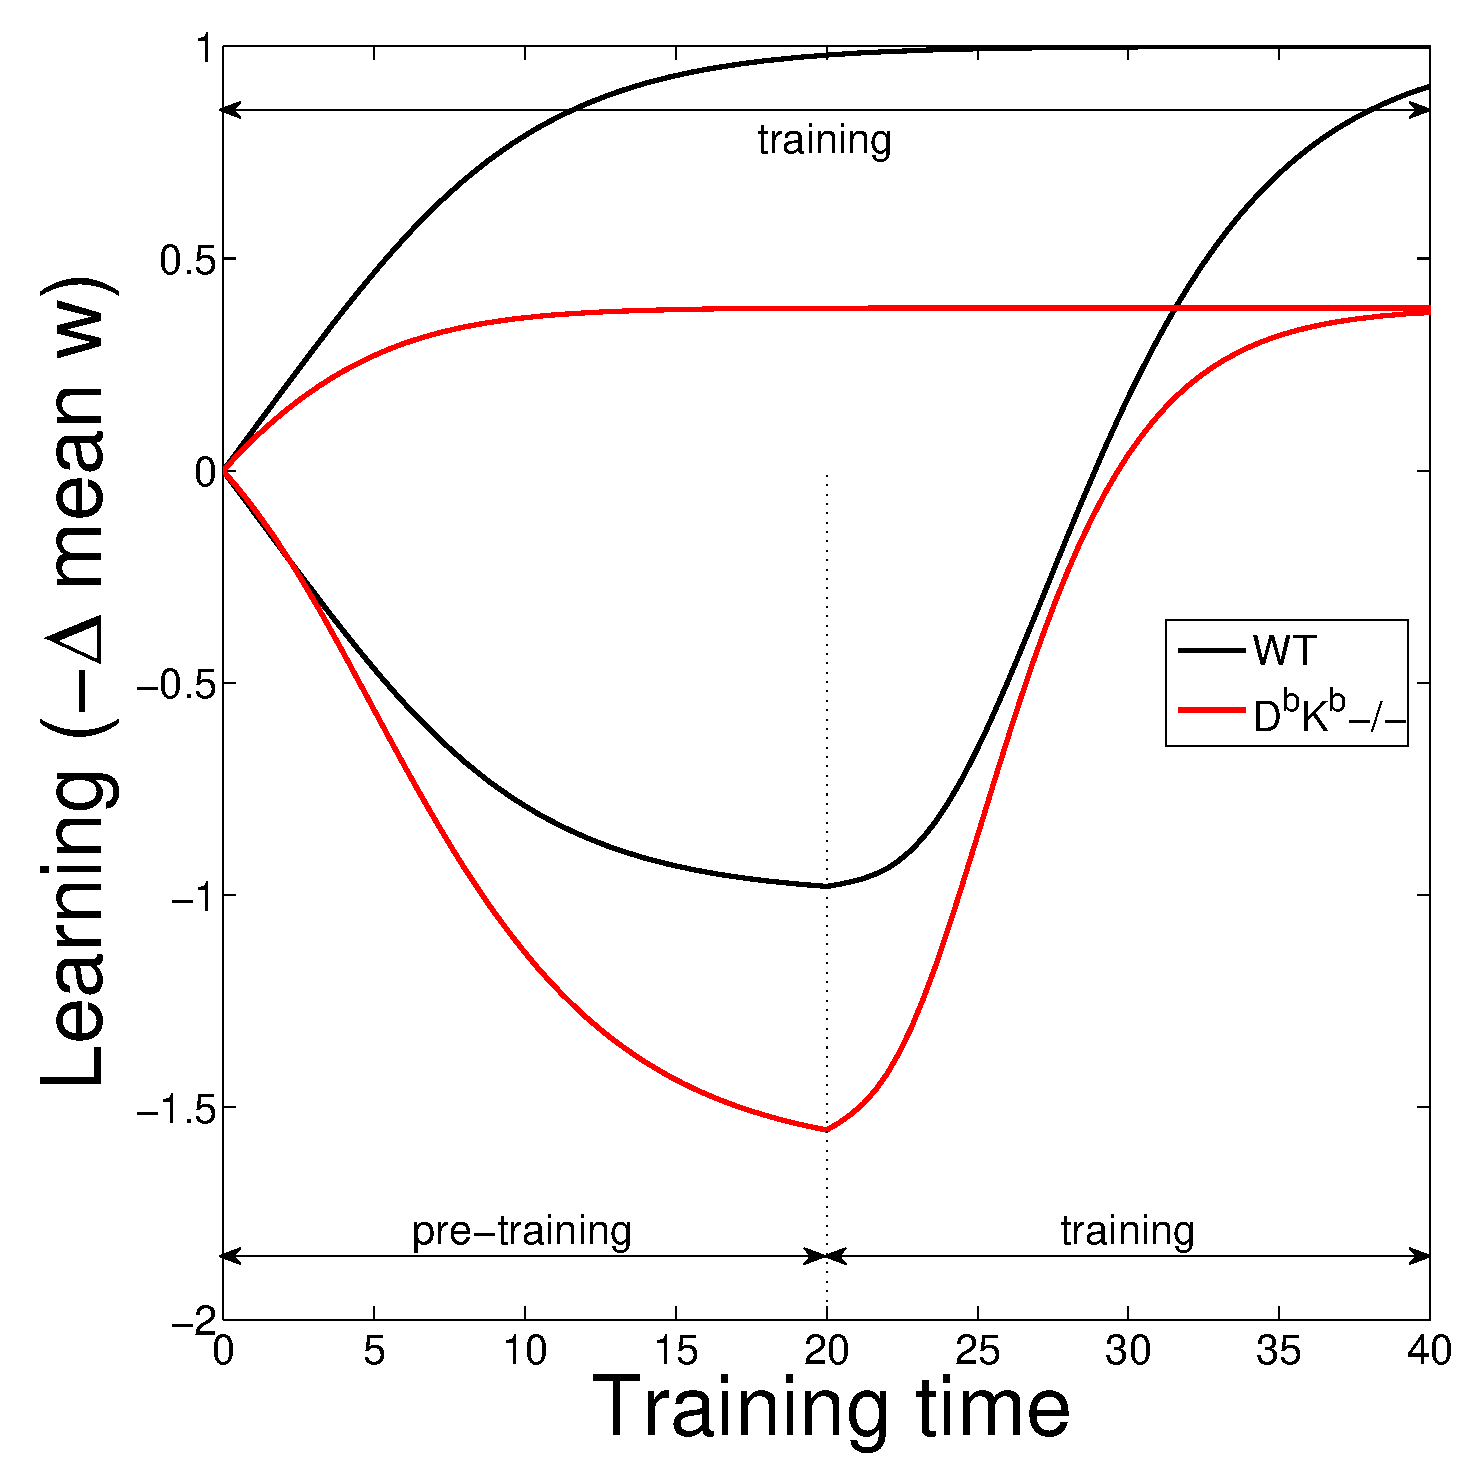
\includegraphics[width=7cm]{multistate_strong_learn.eps}}\label{fig:multistate_strong_learn}
  \item\aligntop{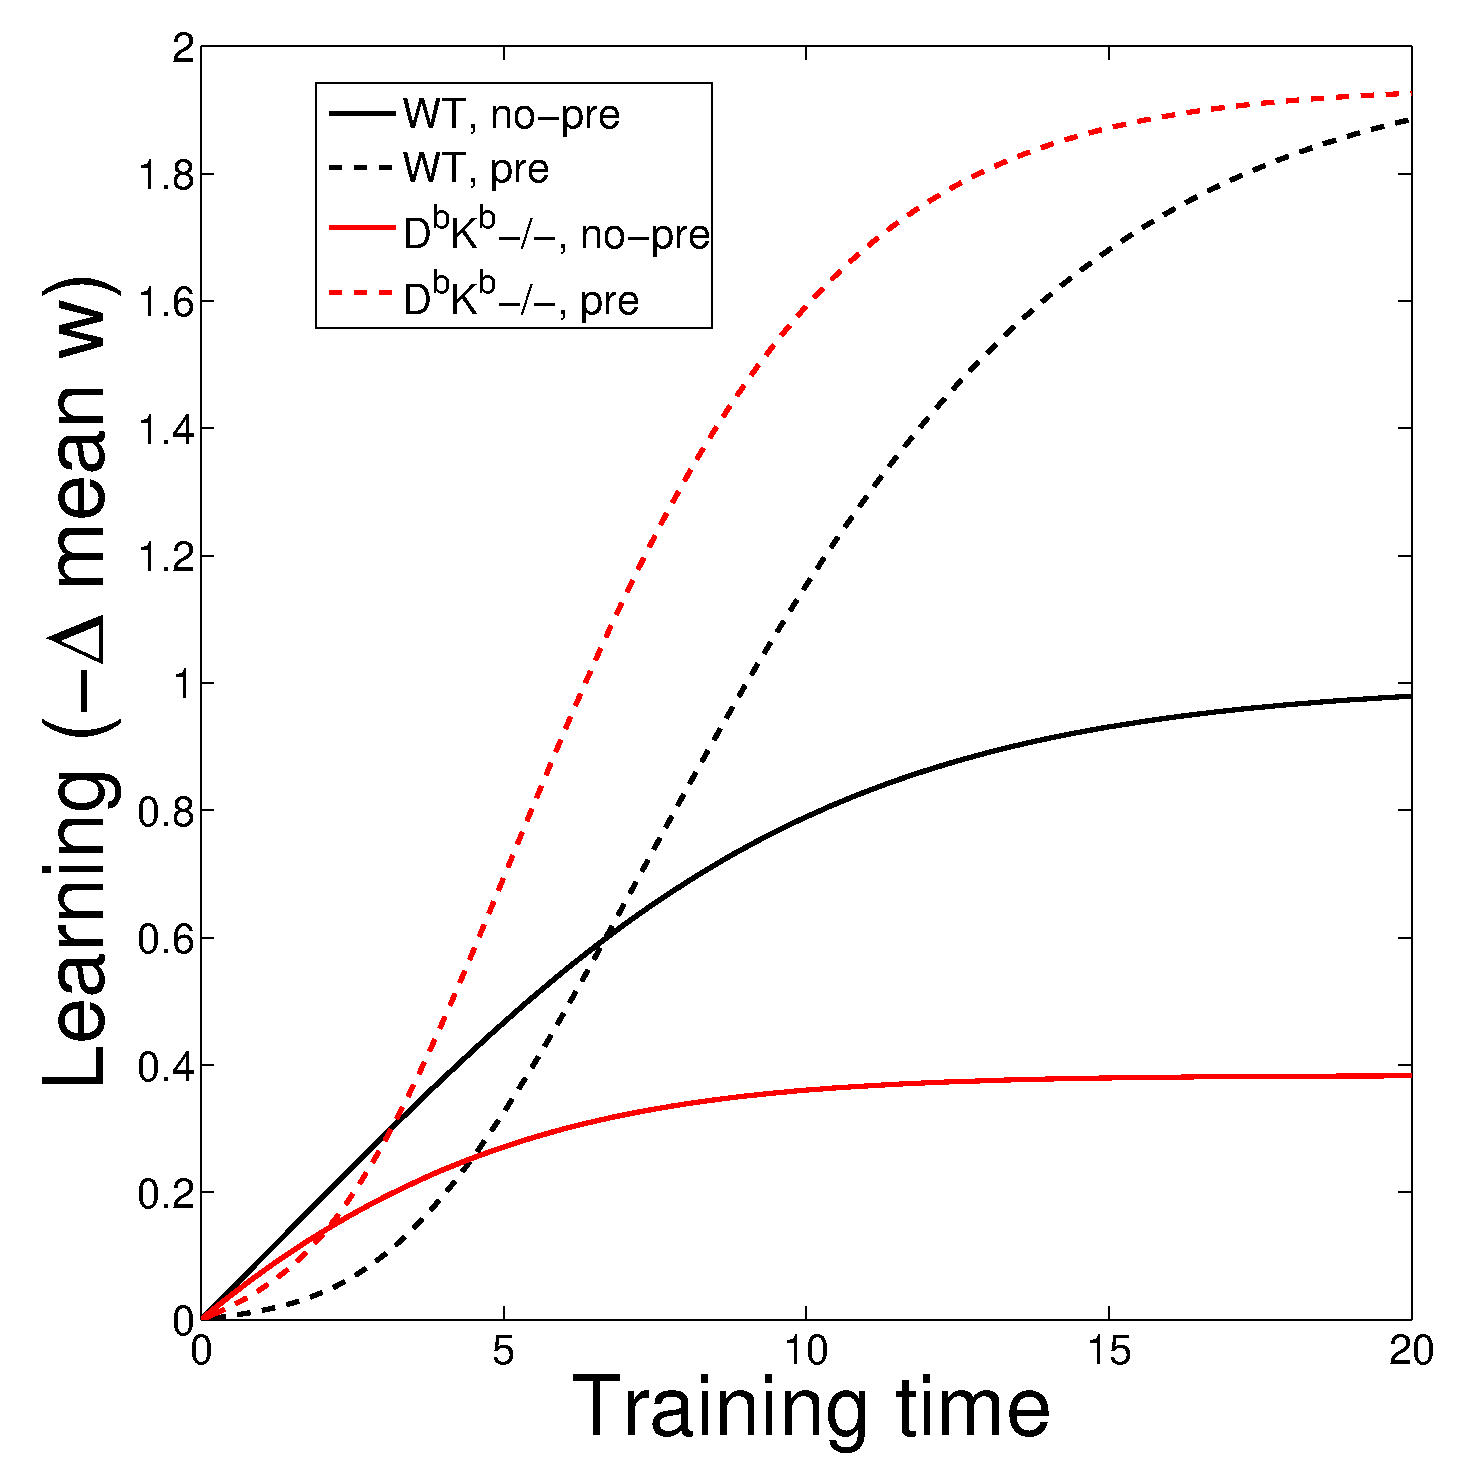
\includegraphics[width=7cm]{multistate_strong_learnS.eps}}\label{fig:multistate_strong_learnS}
  \item\label{fig:multistate_strong_eq}\begin{myenumi}
                    \item\aligntop{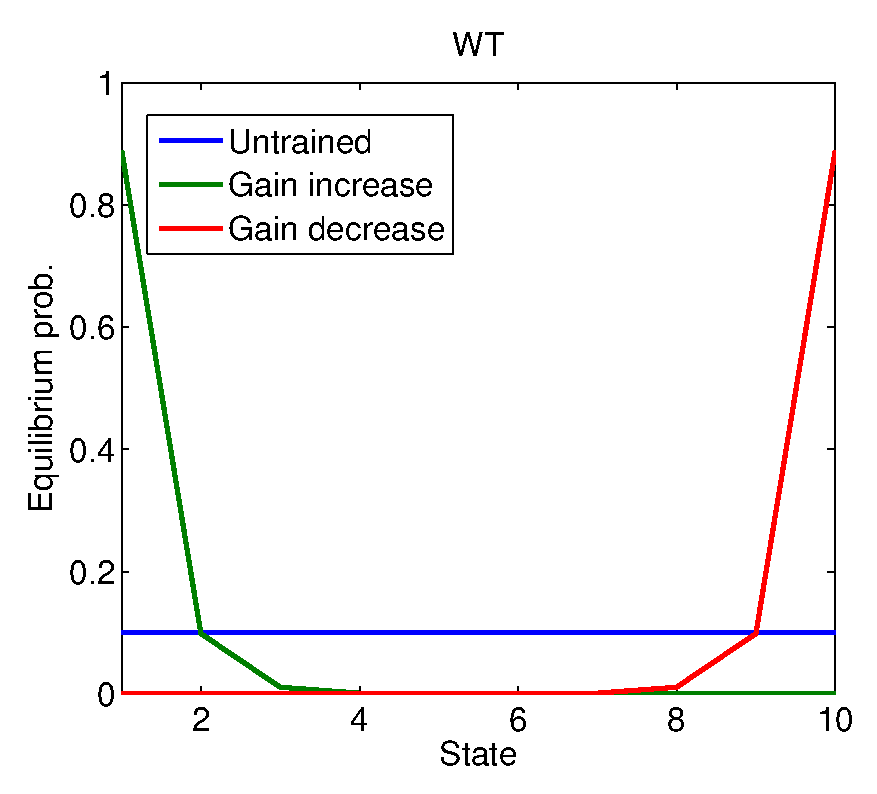
\includegraphics[width=7cm]{multistate_strong_eq_WT.eps}}\label{fig:multistate_strong_eq_WT}
                    \item\aligntop{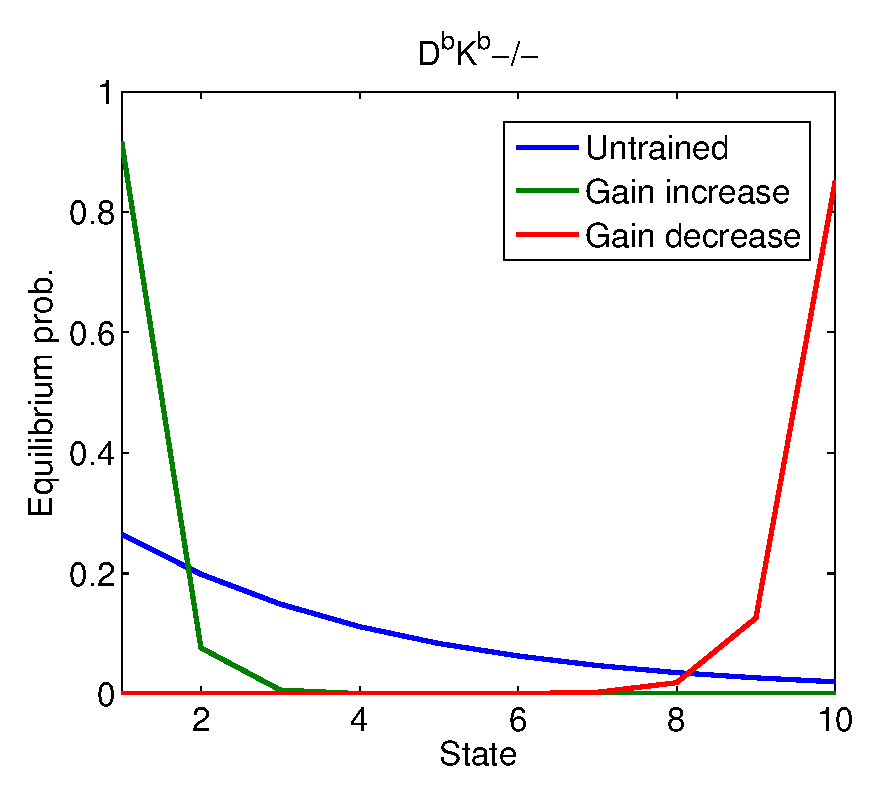
\includegraphics[width=7cm]{multistate_strong_eq_KO.eps}}\label{fig:multistate_strong_eq_KO}
                  \end{myenumi}
  \item\label{fig:multistate_strong_pr}\begin{myenumi}
                    \item\aligntop{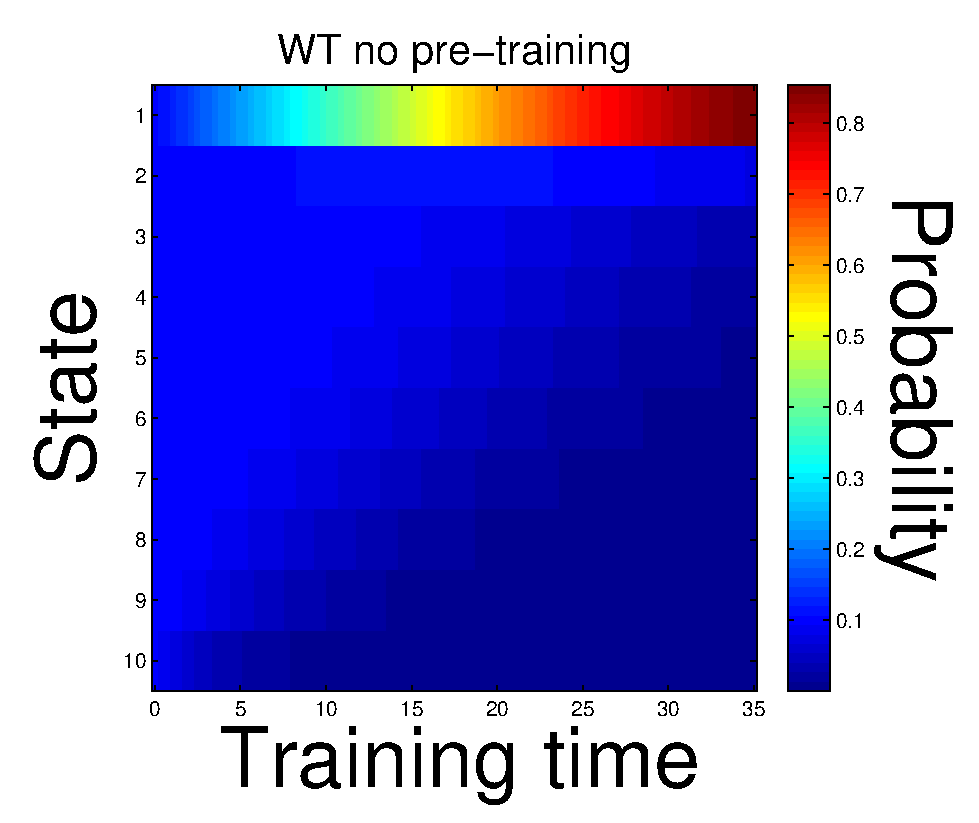
\includegraphics[width=3cm]{multistate_strong_pr_WT_nopre.eps}}\label{fig:multistate_strong_pr_WT_nopre}
                    \item\aligntop{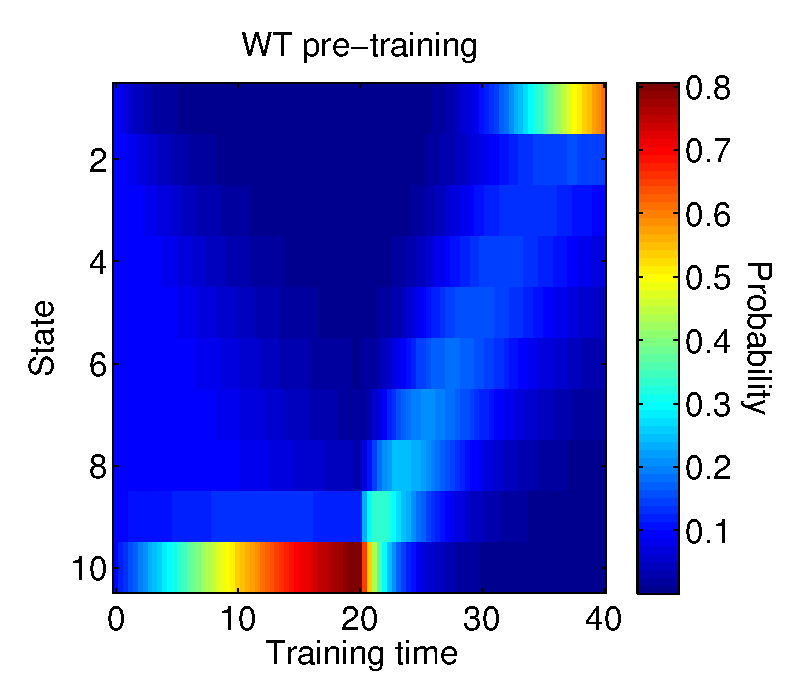
\includegraphics[width=3cm]{multistate_strong_pr_WT_pre.eps}}\label{fig:multistate_strong_pr_WT_pre}
                    \item\aligntop{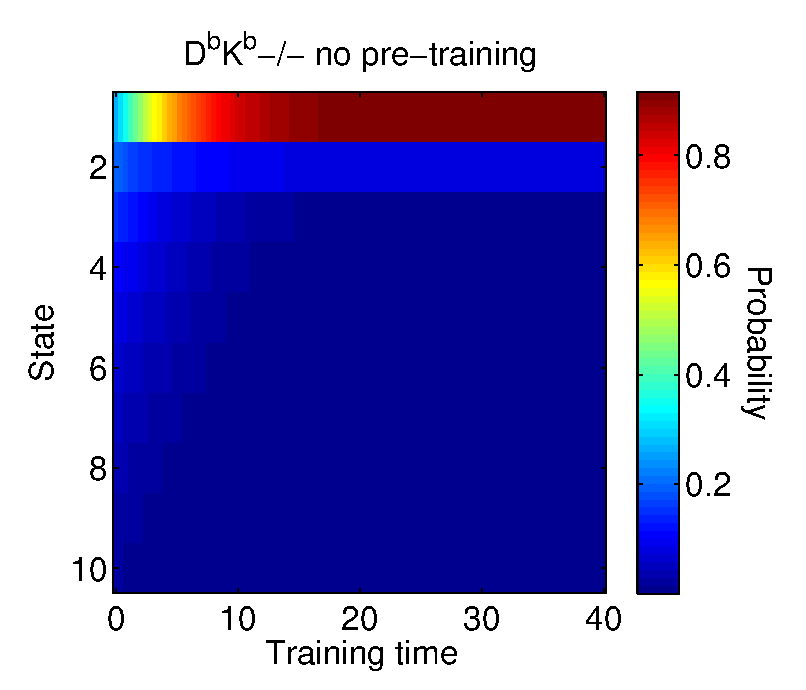
\includegraphics[width=3cm]{multistate_strong_pr_KO_nopre.eps}}\label{fig:multistate_strong_pr_KO_nopre}
                    \item\aligntop{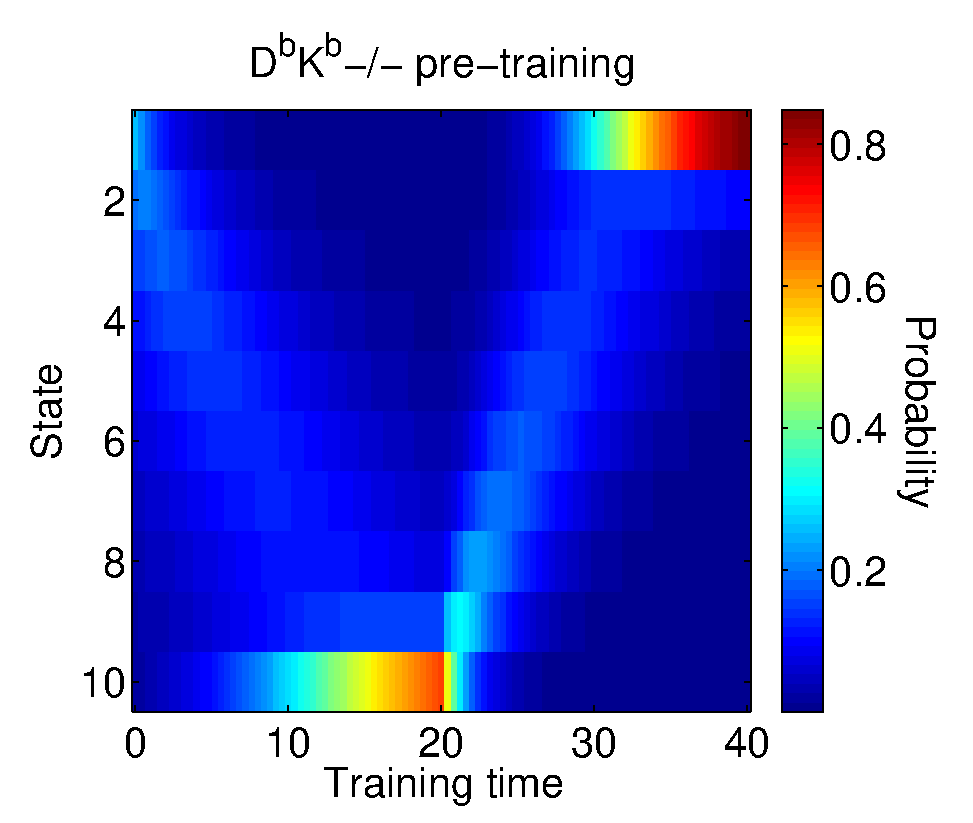
\includegraphics[width=3cm]{multistate_strong_pr_KO_pre.eps}}\label{fig:multistate_strong_pr_KO_pre}
                  \end{myenumi}
 \end{myenuma}
 \end{center}
  \caption{Simulation results for multistate model with strong training ($\Delta f=-0.4$).
  Other parameters can be found in \autoref{tab:params}.
  (\ref{fig:multistate_strong_learn}) Learning curves for wild-type and \KO\ mutant with and without pre-training.
  (\ref{fig:multistate_strong_learnS}) Learning curves restricted to gain-increase training.
  (\ref{fig:multistate_strong_eq}) Equilibrium distributions with/without gain-increase/decrease training for (\ref{fig:multistate_strong_eq_WT}) wild-type and (\ref{fig:multistate_strong_eq_KO}) \KO\ mutant.
  (\ref{fig:multistate_strong_pr}) Evolution of probability distributions for (\ref{fig:multistate_strong_pr_WT_nopre}\ref{fig:multistate_strong_pr_WT_pre}) wild-type and  (\ref{fig:multistate_strong_pr_KO_nopre}\ref{fig:multistate_strong_pr_KO_pre}) \KO\ mutant without (\ref{fig:multistate_strong_pr_WT_nopre},\ref{fig:multistate_strong_pr_KO_nopre}) and with (\ref{fig:multistate_strong_pr_WT_pre},\ref{fig:multistate_strong_pr_KO_pre}) pre-training. } \label{fig:multistate_strong}
\end{figure}

The results of simulations of the multistate model can be seen in \autoref{fig:multistate_weak} and \autoref{fig:multistate_strong}.
However, we can get some insight into this model analytically.



Consider the general uniform multistate model.
Then the equilibrium distribution is given by
%
\begin{equation}\label{eq:mutltieq}
  \eq_i = \frac{1-\alpha}{1-\alpha^M}\,\alpha^{i-1},
  \qquad \text{where} \quad
  \alpha=\frac{f\pot q\pot}{f\dep q\dep}.
\end{equation}
%
If we take the limit $\alpha\rightarrow1$, this becomes $\frac{1}{M}$.

The net-flux from the $\w=+1$ states to the $\w=-1$ states is:
%
\begin{equation}\label{eq:multiflux}
  \Phi = \eq_{M/2+1}f'{}\dep q\dep - \eq_{M/2}f'{}\pot q\pot = \frac{1-\alpha}{1-\alpha^M}\,\alpha^{M/2-1}\prn{\alpha-\alpha'}f'{}\dep q\dep,
\end{equation}
%
where primed values correspond to the new value of $f\pot$.

First, consider the wild-type, for which $q\pot=q\dep=q$.
Without pre-training:
%
\begin{equation}\label{eq:multiWTnopre}
  \Phi = -\frac{2\Delta fq}{M},
\end{equation}
%
where it's worth remembering that $\Delta f<0$.
With pre-training:
%
\begin{equation}\label{eq:multiWTpre}
\begin{aligned}
  \Phi &= 16(\Delta f)^2q \, \frac{(1-2\Delta f)^{M/2-1} (1+2\Delta f)^{M/2-1}}
          {(1-2\Delta f)^M - (1+2\Delta f)^M} \\
       &= -\frac{4\Delta fq}{M} + \CO(\Delta f)^2.
\end{aligned}
\end{equation}
%
So, we see that pre-training will speed up learning when $\Delta f$ is small (in absolute value), as seen in \autoref{fig:multistate_weak}\ref{fig:multistate_weak_learnS}.
On the other hand, if $\Delta f$ is close to $-\half$, pre-training will initially slow down learning a lot, as seen in \autoref{fig:multistate_strong}\ref{fig:multistate_strong_learnS}.

Intuitively, the flux depends on the slope of the distribution at the centre of the chain (with an offset due to the difference between $f\pot$ and $f\dep$).
Pre-training has two effects: it produces a slope in the right direction (see \autoref{fig:multistate_weak}\ref{fig:multistate_weak_eq}), but it also reduces distribution at the centre (see \autoref{fig:multistate_strong}\ref{fig:multistate_strong_eq}).
For small $\Delta f$, the first effect is stronger and learning speeds up.
For larger $\Delta f$, the second effect wins and learning slows down.

Now, consider the mutant, for which $q\pot=\beta q\dep=q$, $\beta<1$.
Without pre-training:
%
\begin{equation}\label{eq:multiKOnopre}
  \Phi = -2\Delta f q\,\frac{(1-\beta)\beta^{M/2-1}}{1-\beta^M}.
\end{equation}
%
This will be smaller than \eqref{eq:multiWTnopre} if $\beta<\beta^*(M)$.
This function is plotted in \autoref{fig:multistate_star}\ref{fig:multistate_betastar}, where we can see that it approaches 1 rapidly as we increase $M$.

There are two effects here as well.
Smaller $\beta$ will increase the probability of crossing the centre of the chain, speeding up learning, but it will also concentrate probability at the ends of the chain, depleting the centre and slowing down learning.
The first effect goes like $1/\beta$, whereas the second goes like $\beta^{M/2}$ and will be more significant for smaller $\beta$ or in a longer chain.

With pre-training:
%
\begin{equation}\label{eq:multiKOpre}
\begin{aligned}
  \Phi &= -4\Delta f q \, \frac{(1-2\Delta f) - \beta(1+2\Delta f)}
          {(1-2\Delta f)^M - \beta^M(1+2\Delta f)^M}   \,
          \beta^{M/2-1}(1-2\Delta f)^{M/2-1} (1+2\Delta f)^{M/2-1} \\
       &= -4\Delta f q\,\frac{(1-\beta)\beta^{M/2-1}}{1-\beta^M} + \CO(\Delta f)^2.
\end{aligned}
\end{equation}
%
Once again, we see that pre-training will speed up learning when $\Delta f$ is small, whereas, if $\Delta f$ is close to $-\half$, pre-training will initially slow down learning.

Let us define $\Delta f^*(\beta,M)$ to be the value at which \eqref{eq:multiKOnopre} and \eqref{eq:multiKOpre} are equal.
As we would like pre-training to slow down learning in the wild-type but speed it up in the mutant, it would seem that we require $\Delta f^*(\beta,M) < \Delta f < \Delta f^*(1,M)$ (remembering once more that $\Delta f<0$ and that the wild-type corresponds to $\beta=1$).
However, as seen in \autoref{fig:multistate_star}\ref{fig:multistate_deltafstar}, $\Delta f^*(\beta,M) > \Delta f^*(1,M)$, which would make this impossible.

But, all is not lost.
This is only the initial, instantaneous rate of change.
Let's look at \autoref{fig:multistate_strong}\ref{fig:multistate_strong_learnS}, for which $\Delta f < \Delta f^*(1,M)$, so that pre-training initially slows down learning for both wild-type and mutant.
We see that the pre-trained curve can rapidly catch up with the un-pre-trained one, due to the mass of probability concentrated at the end of the chain (see \autoref{fig:multistate_strong}\ref{fig:multistate_strong_eq}) drifting to the centre.
This happens sooner for the mutant than the wild-type, due to the stronger depressing transitions.
This means that there is an intermediate range of time-scales over which pre-training does slow down learning in the wild-type but speed it up in the mutant.

In conclusion, if we choose $\beta<\beta^*(M)$, $\Delta f < \Delta f^*(1,M)$ and look at intermediate time-scales, we will see that the mutant learns slower than wild-type without pre-training, and that pre-training speeds up learning in the mutant but slows it down in the wild-type.
However, in this case pre-training proceeds much faster in the mutant than wild-type (see \autoref{fig:multistate_strong}\ref{fig:multistate_strong_learn}), which is \emph{not} seen in the experiment.



\begin{figure}
 \begin{center}
 \begin{myenuma}
  \item\aligntop{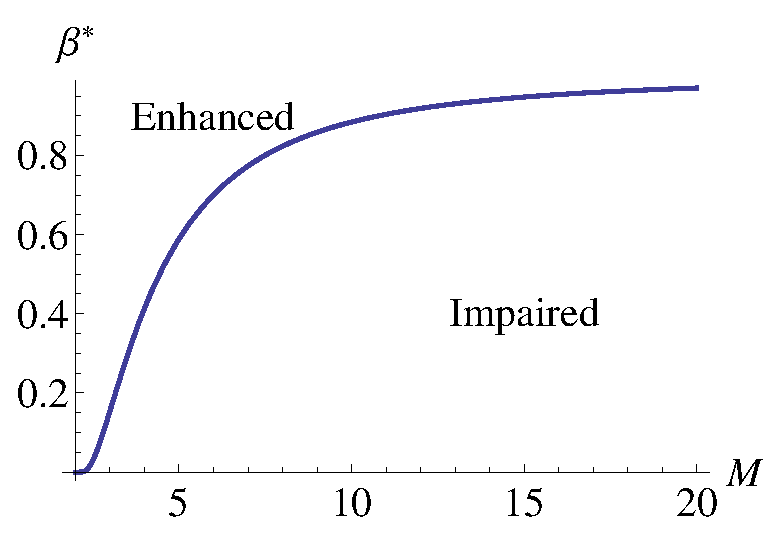
\includegraphics[width=7cm]{multistate_betastar.eps}}\label{fig:multistate_betastar}
  \item\aligntop{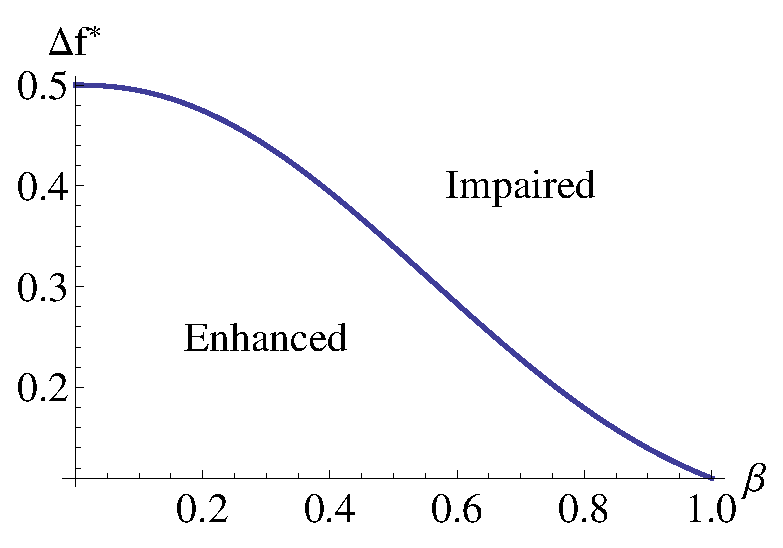
\includegraphics[width=7cm]{multistate_deltafstar.eps}}\label{fig:multistate_deltafstar}
 \end{myenuma}
 \end{center}
  \caption{The functions (\ref{fig:multistate_betastar}) $\beta^*(M)$ and (\ref{fig:multistate_deltafstar}) $\Delta f^*(\beta,M)$ for $M=10$.}\label{fig:multistate_star}
\end{figure}



\subsubsection{Two-state model}\label{sec:binary}

\begin{figure}
 \begin{center}
 \begin{myenuma}
  \item\aligntop{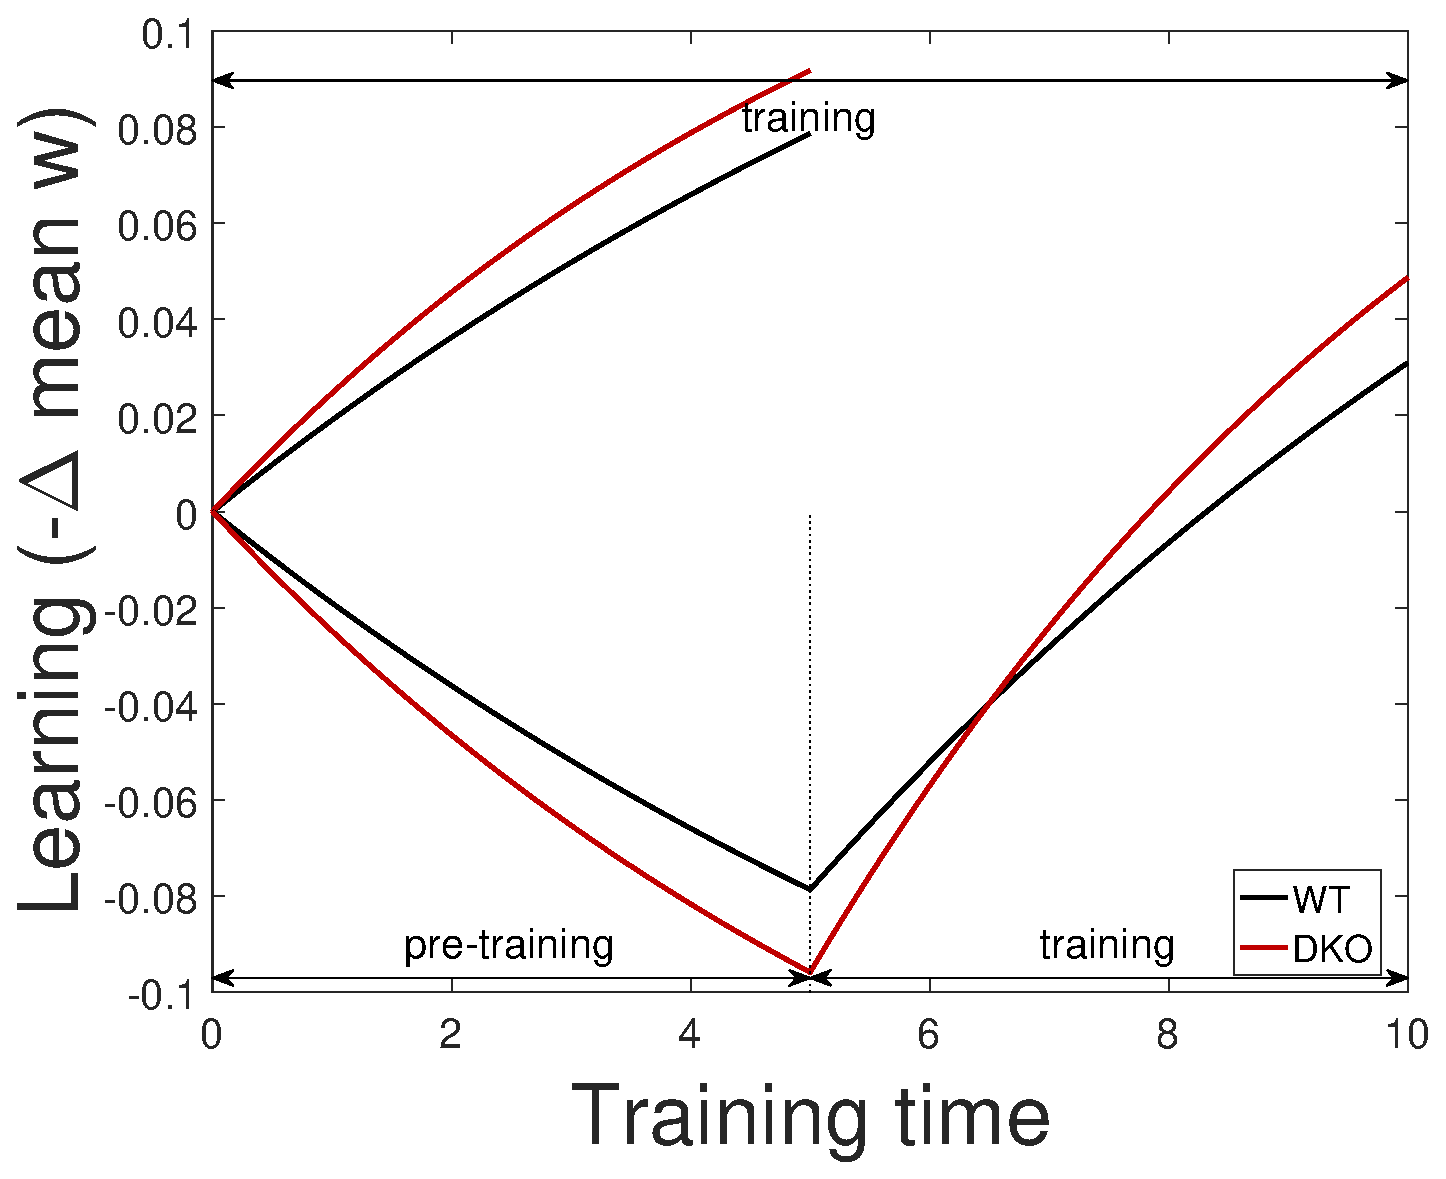
\includegraphics[width=7cm]{binary_learn.eps}}\label{fig:binary_learn}
  \item\aligntop{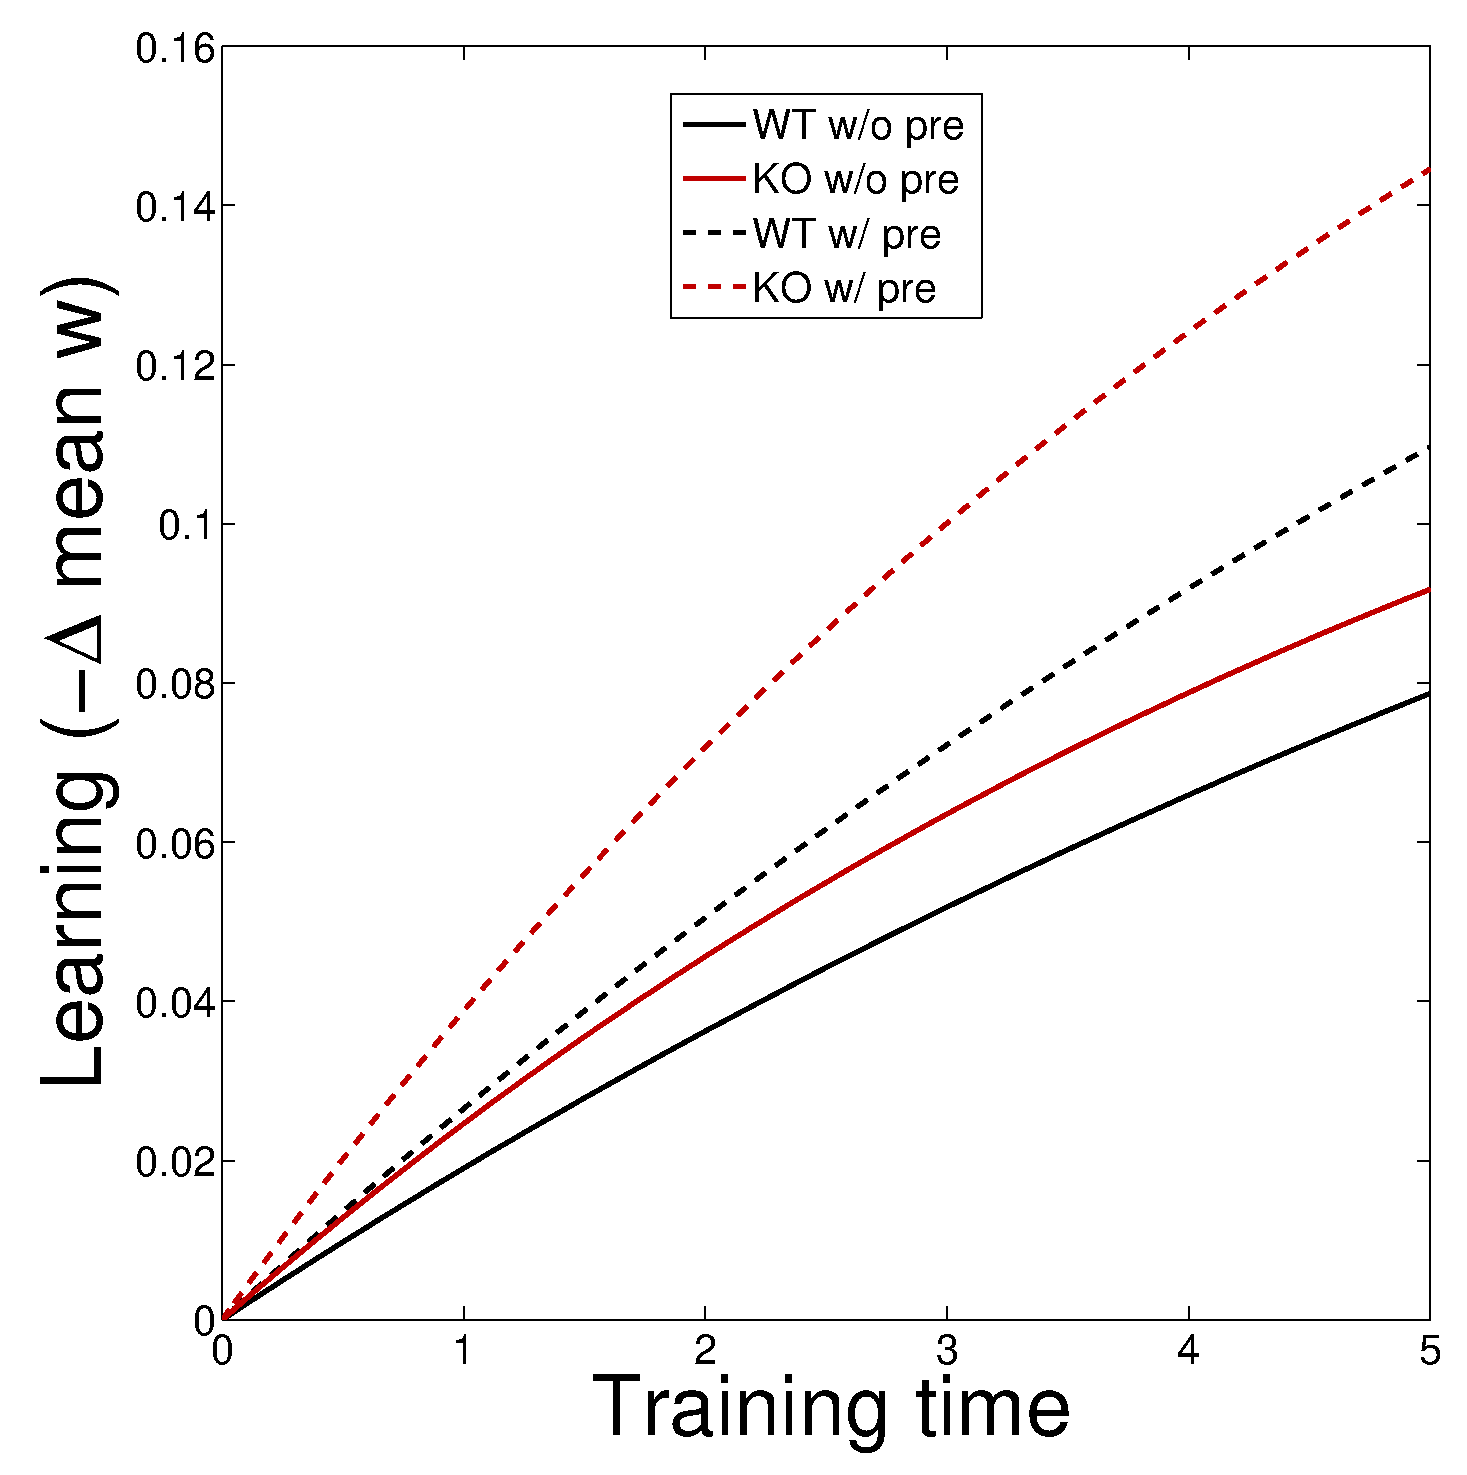
\includegraphics[width=7cm]{binary_learnS.eps}}\label{fig:binary_learnS}
  \item\label{fig:binary_eq}\begin{myenumi}
                    \item\aligntop{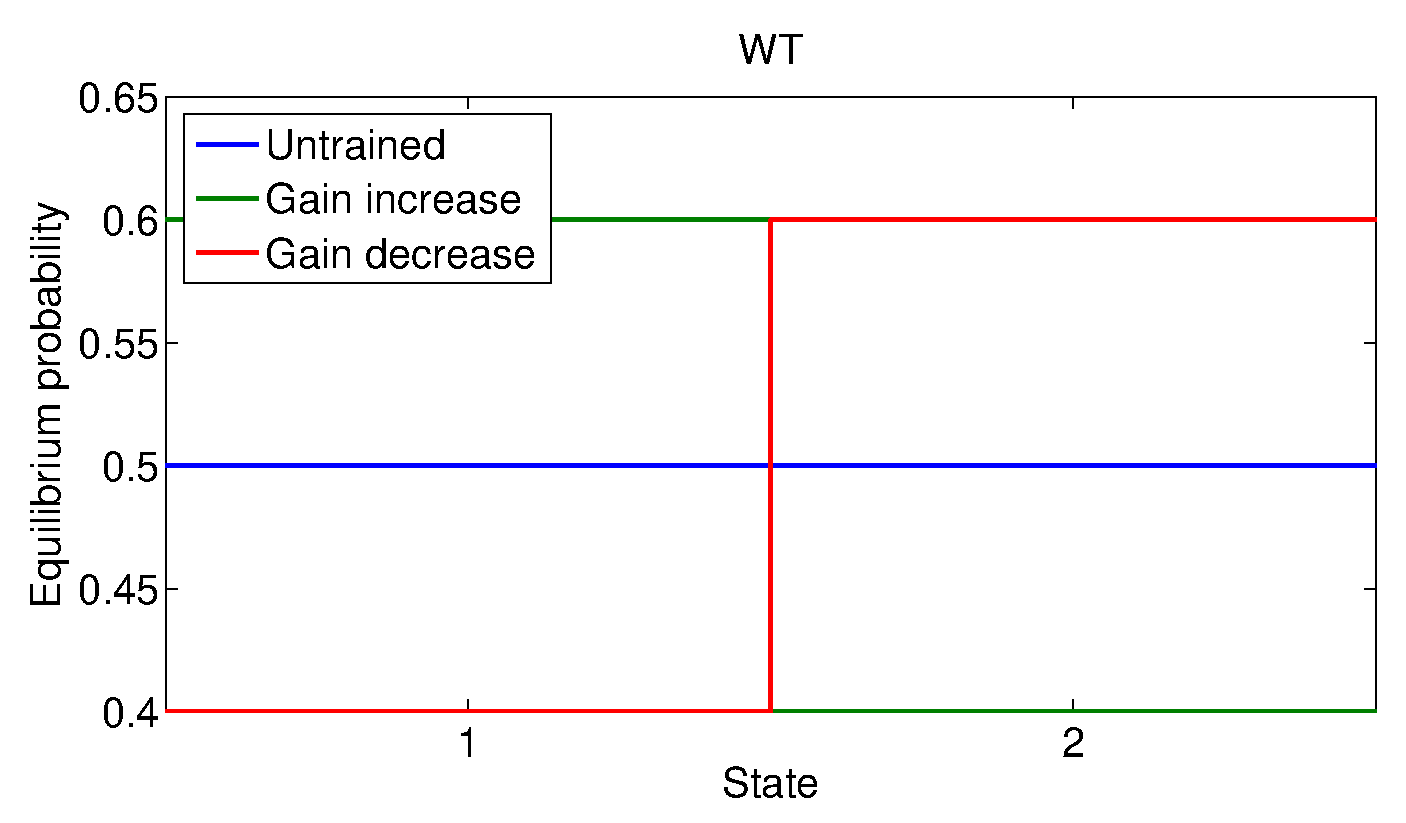
\includegraphics[width=7cm]{binary_eq_WT.eps}}\label{fig:binary_eq_WT}
                    \item\aligntop{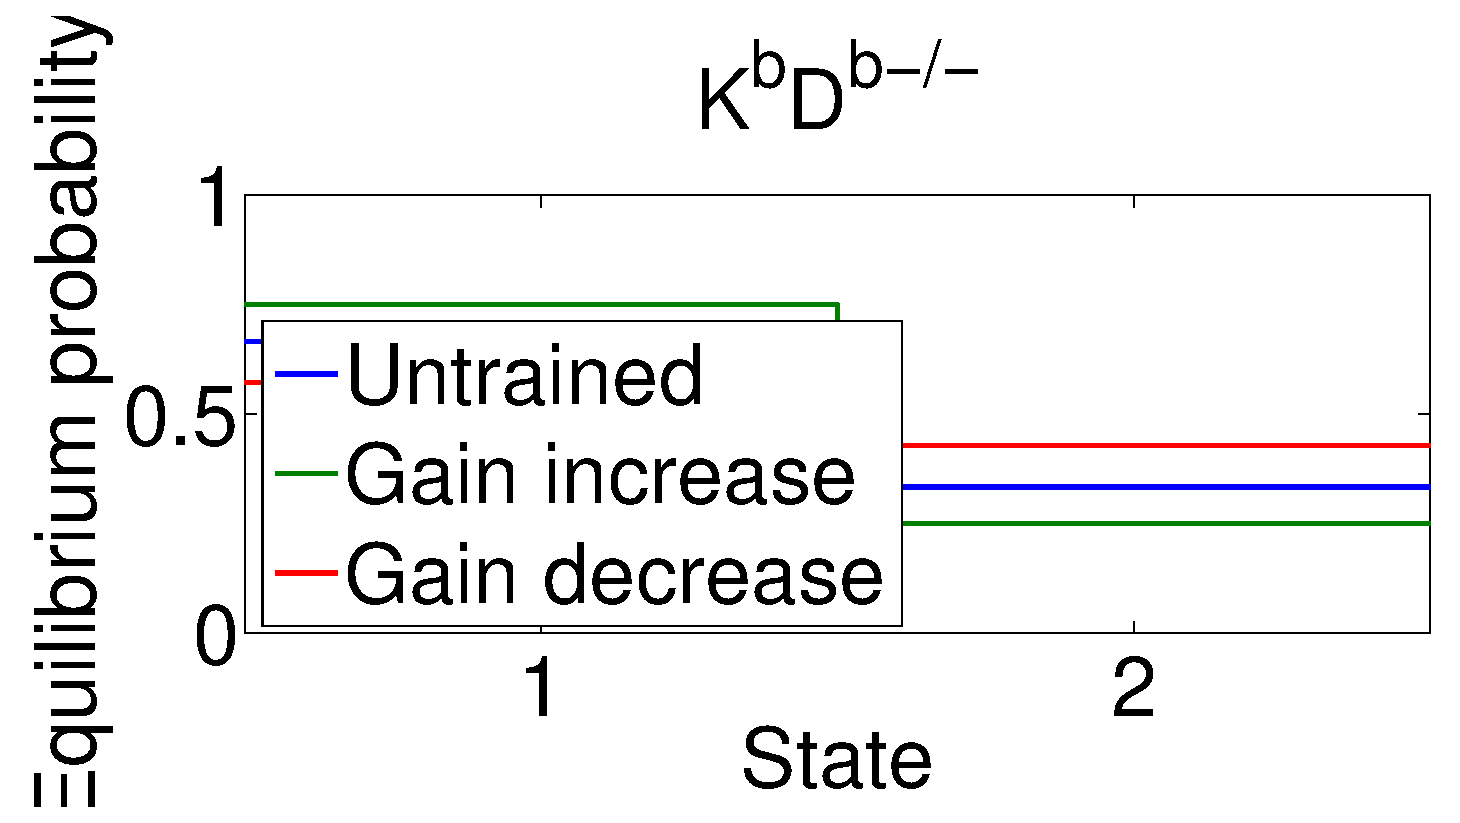
\includegraphics[width=7cm]{binary_eq_KO.eps}}\label{fig:binary_eq_KO}
                  \end{myenumi}
  \item\label{fig:binary_pr}\begin{myenumi}
                    \item\aligntop{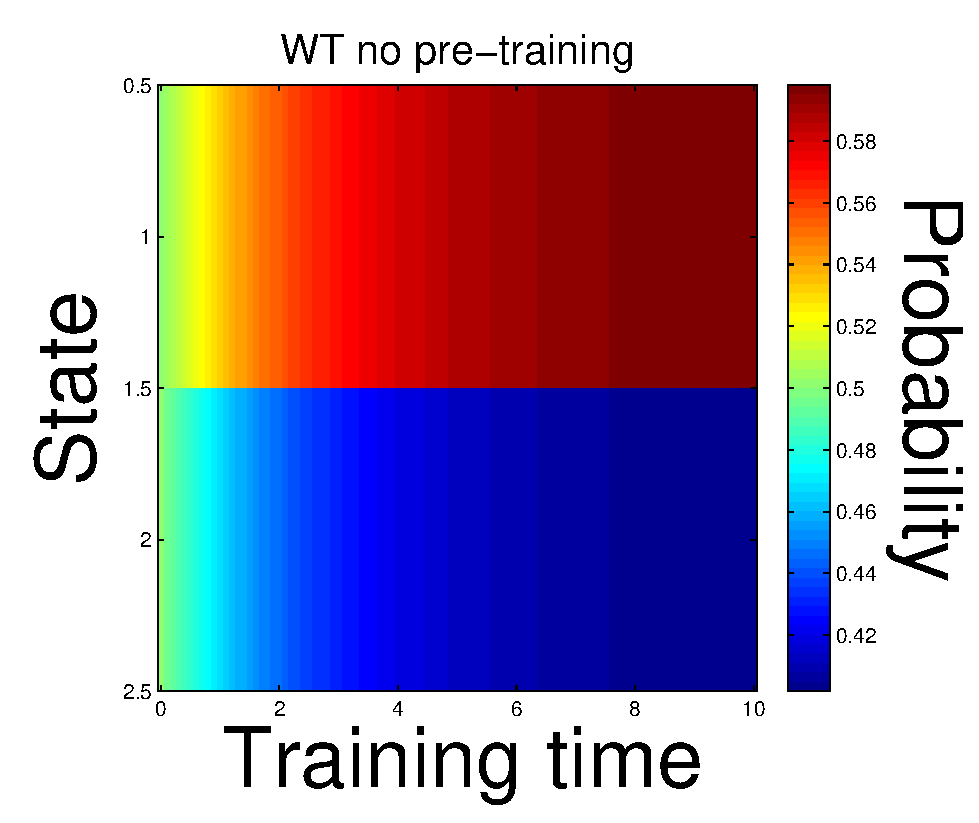
\includegraphics[width=3cm]{binary_pr_WT_nopre.eps}}\label{fig:binary_pr_WT_nopre}
                    \item\aligntop{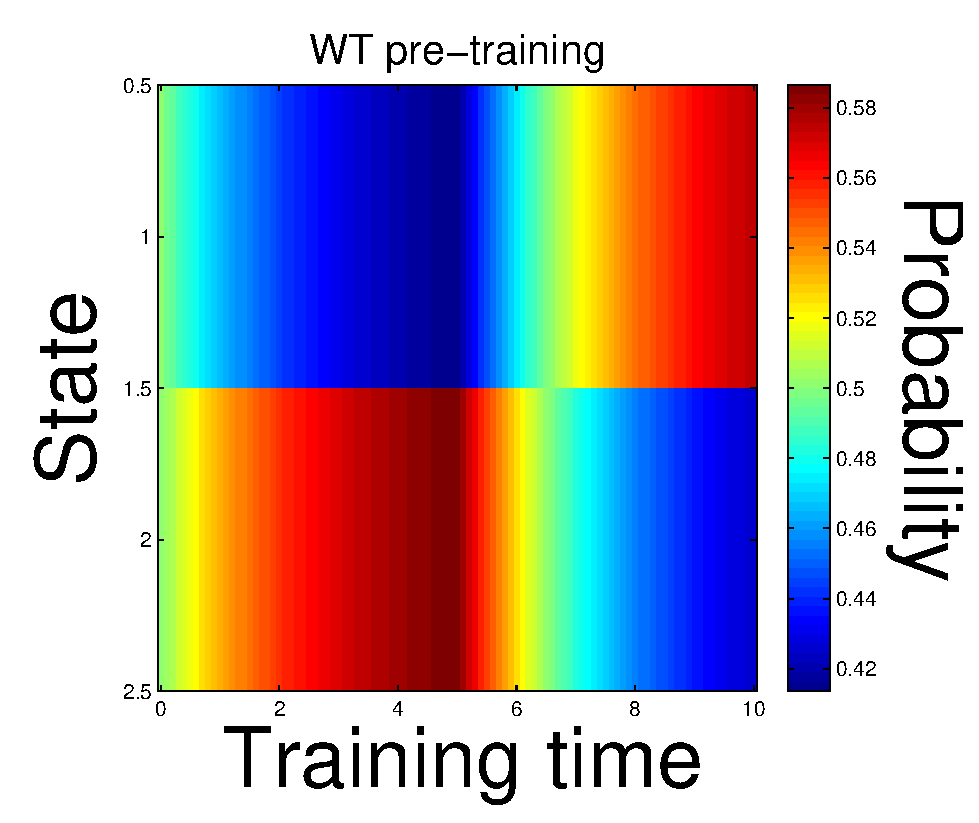
\includegraphics[width=3cm]{binary_pr_WT_pre.eps}}\label{fig:binary_pr_WT_pre}
                    \item\aligntop{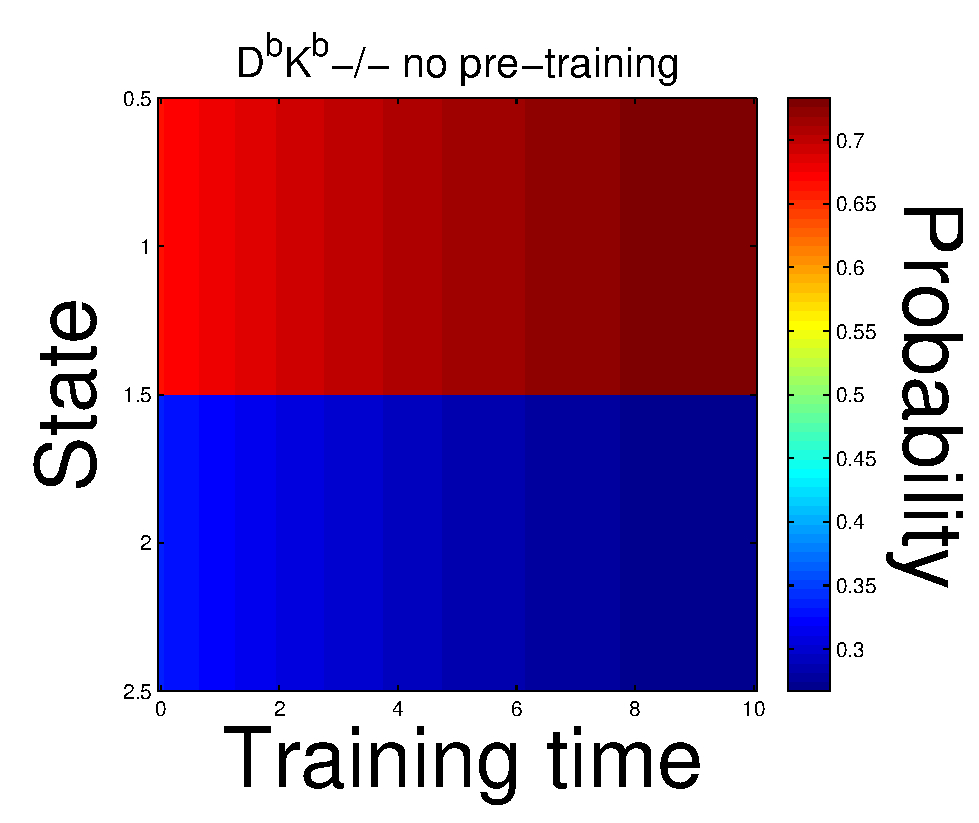
\includegraphics[width=3cm]{binary_pr_KO_nopre.eps}}\label{fig:binary_pr_KO_nopre}
                    \item\aligntop{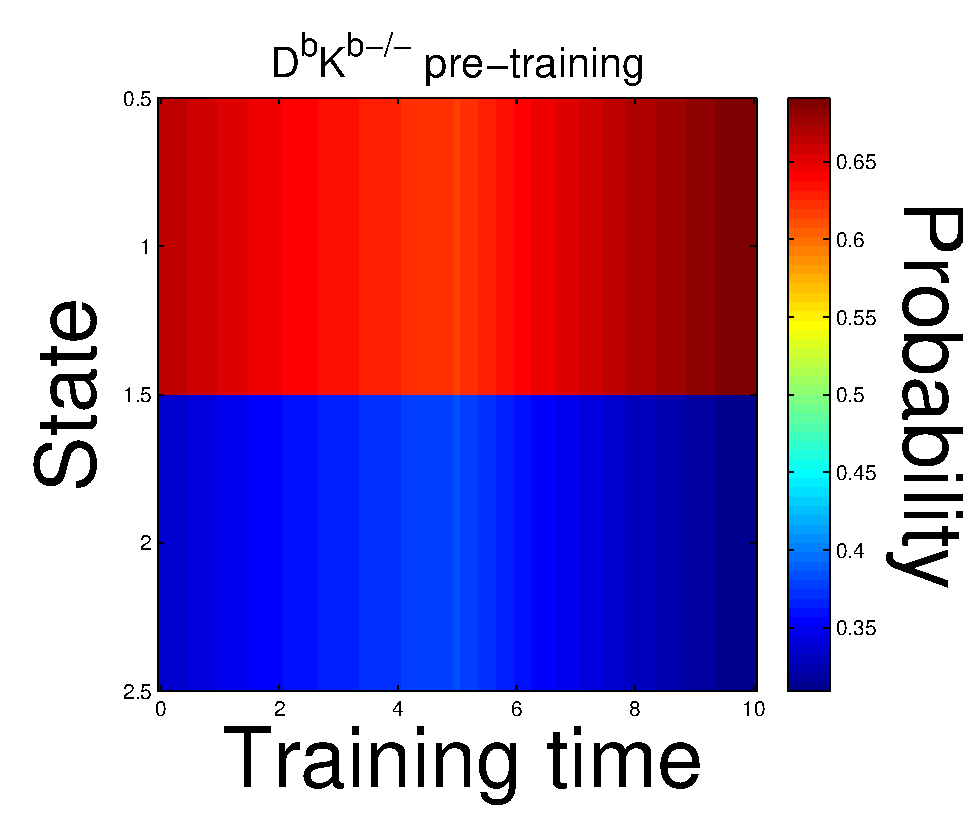
\includegraphics[width=3cm]{binary_pr_KO_pre.eps}}\label{fig:binary_pr_KO_pre}
                  \end{myenumi}
 \end{myenuma}
 \end{center}
  \caption{Simulation results for two-state model.
  Parameters can be found in \autoref{tab:params}.
  (\ref{fig:binary_learn}) Learning curves for wild-type and \KO\ mutant with and without pre-training.
  (\ref{fig:binary_learnS}) Learning curves restricted to gain-increase training.
  (\ref{fig:binary_eq}) Equilibrium distributions without training or with gain-increase/decrease training for (\ref{fig:binary_eq_WT}) wild-type and (\ref{fig:binary_eq_KO}) \KO\ mutant.
  (\ref{fig:binary_pr}) Evolution of probability distributions for (\ref{fig:binary_pr_WT_nopre}\ref{fig:binary_pr_WT_pre}) wild-type and  (\ref{fig:binary_pr_KO_nopre}\ref{fig:binary_pr_KO_pre}) \KO\ mutant without (\ref{fig:binary_pr_WT_nopre},\ref{fig:binary_pr_KO_nopre}) and with (\ref{fig:binary_pr_WT_pre},\ref{fig:binary_pr_KO_pre}) pre-training. } \label{fig:binary_res}
\end{figure}


The results of simulations of the multistate model can be seen in \autoref{fig:binary_res}.
However, this model can be solved exactly:
%
\begin{multline}\label{eq:binarysol}
  \eq = \frac{(f\dep q\dep, f\pot q\pot)}{\lambda},
  \qquad
  \pr(t) = \eq + (\pr(t)-\eq)\e^{-\lambda rt},\\
  \qquad \text{where} \quad
  \lambda = f\pot q\pot + f\dep q\dep.
\end{multline}
%
But it is easier to just substitute $M=2$ into the formulae in \sref{sec:multistate}.
In this case, the initial rate of change encapsulates the whole solution, as there is only a single exponential decay.

First, consider the wild-type, for which $q\pot=q\dep=q$.
Without pre-training:
%
\begin{equation}\label{eq:binWTnopre}
  \Phi = -\Delta f q,
\end{equation}
%
where, again, it's worth remembering that $\Delta f<0$.
With pre-training:
%
\begin{equation}\label{eq:binWTpre}
\begin{aligned}
  \Phi &= -2\Delta f q.
\end{aligned}
\end{equation}
%
So, we see that pre-training will always speed up learning, unlike what is seen in the experiment.
This can be seen in \autoref{fig:binary_res}\ref{fig:binary_learn},\ref{fig:binary_learnS}.

Now, consider the mutant, for which $q\pot=\beta q\dep=q$, $\beta<1$.
Without pre-training:
%
\begin{equation}\label{eq:binKOnopre}
  \Phi = -\frac{2\Delta f q}{1+\beta},
\end{equation}
%
which is always larger that \eqref{eq:binWTnopre}, unlike what is seen in the experiment.
This is also seen in \autoref{fig:binary_res}\ref{fig:binary_learn},\ref{fig:binary_learnS}.
As discussed below \eqref{eq:multiKOnopre}, the smaller values of has two effects.
Smaller $\beta$ will increase the probability of depression, speeding up learning, but it will also decrease the probability of being ready for depression, slowing down learning.
The second effect is much smaller for the very short chain considered here.

With pre-training:
%
\begin{equation}\label{eq:binKOpre}
\begin{aligned}
  \Phi &= -4\Delta f q \, \frac{(1-2\Delta f) - \beta(1+2\Delta f)}
          {(1-2\Delta f)^2 - \beta^2(1+2\Delta f)^2}.
\end{aligned}
\end{equation}
%
As we've already ruled out this model, we won't waste any time analysing this formula.


\subsubsection{Pooled resource model}\label{sec:pooled}



%\subsection*{Acknowledgements}



%%%%%%%%%%%%%%%%%%%%%%%%%%%%%%%%%%%%%%%%%%%%%%%%%%%%%%%%%%%%%%%%%%%%%%%%%%
%\subsection*{Appendices}
%\appendix
%%%%%%%%%%%%%%%%%%%%%%%%%%%%%%%%%%%%%%%%%%%%%%%%%%%%%%%%%%%%%%%%%%%%%%%%%%





%%%%%%%%%%%%%%%%%%%%%%%%%%%%%%%%%%%%%%%%%%%%%%%%%%%%%%%%%%%%%%%%%%%%%%%%%%

\bibliographystyle{utcaps_sl}
\bibliography{maths,neuro}

\end{document}
